%ch03.tex

%\pagestyle{headings}

\chapter{Attribute Enabled Software Development}
\label{ch:gaast}
\label{ch03}
\mquote{We don't usually consider a statement to be data at
all, since it cannot be read, written, or manipulated.}{R. A. Finkel, Advanced Programming Language Design, 1996}

\noindent This chapter\footnote{This chapter shares content with references \cite{cepa.mezini.gaast.04,cepa.kloppenburg.05}.} explains the main ideas behind attribute-enabled language technologies\footnote{The term \textit{language technology} is used to mean the complete language system: the grammar, the binary representation, and the run-time system.} and their usage to sustain domain specific abstractions (DSA). \Sr{c2.sec.dsa.attributes} portrays how DSA can be supported with attributes, and how the domain variability can be modeled as nested attribute-families. The advantages of \textit{attribute enabled programming} (AEP) are discussed in \sr{sec:gaast-mda}, by analyzing several scenarios for mapping of Model-Driven Architecture (MDA) UML class diagram models onto source code artifacts. %Several widely used approaches for mapping MDA models are compared with the attribute programming.

\Sr{sec:problem-statement} investigates several ways to support the attribute-based software design in UML class diagrams. The language technology behind AEP is discussed in \sr{sec:gaast}, stressing the importance that this technology be part of the core language, and supported by the language vendor. Related approaches are addressed in \sr{sec.related.dsl}. Attribute programming is compared with other ways to support EDSL constructs, namely extensible grammars / compilers and meta-programming systems. Finally, \sr{sec.attribute.usage} explores the proper usage of attributes to clarify the power and some of the pitfalls of the AEP.

\begin{figure}[ht]
%	\begin{center}
	  \xymatrix{
	  *+[F]{\txt{Supporting DSA with Attributes \\\Sr{c2.sec.dsa.attributes}}} \ar[r] \ar[d] \ar[dr] &
	  *+[F]{\txt{GAAST Languages \\\Sr{sec:gaast}}} \ar[d]
	  \\
	  	*+[F]{\txt{Advantages of Attribute Programming \\\Sr{sec:gaast-mda}}} \ar[d] \ar[dr] & *+[F]{\txt{Comparison to other Approaches  \\\Sr{sec.related.dsl}}}\\  	
*+[F]{\txt{Representing Attributes in UML \\\Sr{sec:problem-statement}}}  	 & *+[F]{\txt{Proper Usage of Attributes \\\Sr{sec.attribute.usage}}} \\  }
%	\end{center}
%	\caption{Chapter Overview}
%	\label{fig:contents}
\end{figure}

\section{Supporting DSA with Attributes}
\label{c2.sec.dsa.attributes}

Based on the third alternative for implementing domain specific abstractions (DSA) explained in \sr{sec:var.dsa}, namely generic language extensions, this book presents technology that addresses the DSA drawbacks mentioned in \sr{sec:var.dsa}, based on \textit{explicit attributes} \cite{hedin.97,java.explicit.programming}. Explicit attributes are a lightweight language extension which reduces the grammar processing costs, and the accidental \cite{brooks.87} costs of the DSA implementation.
%
Using a \textit{attribute} (or \textit{tag}) to denote an additional property about an existing entity is intuitive. When Knuth \cite{knuth.90} describes the idea of using attributes as tags that carry out semantics related to grammar productions, he notes that the idea has been around for some time. Since then, attribute grammars have evolved and matured and they are used in different ways to develop software \cite{attrib.gram}.

\begin{figure}[ht]
	\begin{center}
		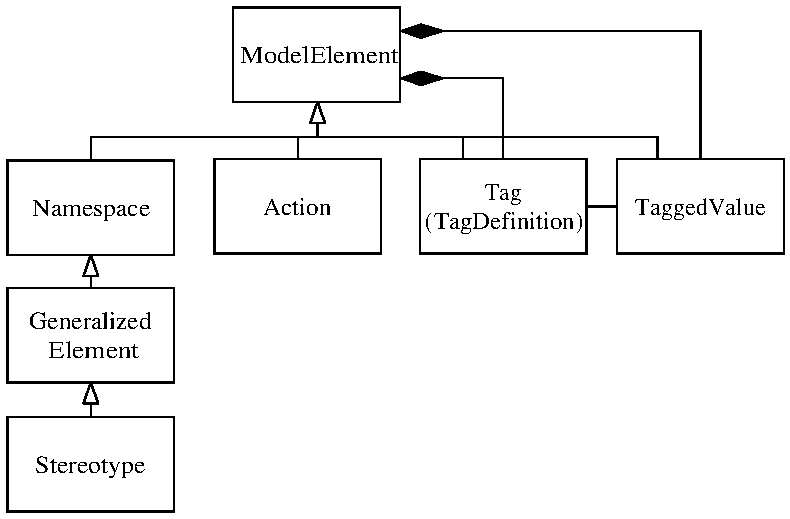
\includegraphics[width=!,height=5cm]{ch03/mof-uml-tag}
	\end{center}
	\caption{The \textit{Tag} element in MOF / UML can be used with any \textit{ModelElement}}
	\label{fig:mof-uml-tag}
\end{figure}

An example is the tag definition and usage in the Meta-Object Facility (MOF) \cite{www.mof} and the Unified Modeling Language (UML) \cite{www.uml}\footnote{UML can be described in terms of MOF.}. In MOF, tags derive from the class {\tt Mo\-del\-Ele\-ment}, i.e., any element can be decorated with custom defined tags (\fig{fig:mof-uml-tag}). Tags carry no domain-specific semantics for the MOF or UML itself. Their semantics are meaningful only to the modeler of the profile, who introduces the tag definitions. Tags serve as hints to model transformers and generators \cite{mda.frankel}, and enable the association of arbitrary semantics with model elements of interest, without having to change the meta-model of a given model. In terms of MOF, tags enable modeling in different vertical layers simultaneously. There is some functionality available to modify the meta-model M$_{i+1}$ in the layer M$_{i}$, providing similar functionality in the layer M$_{i}$, as found directly in the upper meta-model layer M$_{i+1}$. 

This book focuses on the usage of \textit{attributes} \cite{www.dotnet}, known also as \textit{annotations} \cite{www.java.meta}, or \textit{tags} \cite{www.mof}, as a form of graph labeling \cite{term.rewrite,Plump.95,mens.99} at the programming language level\footnote{Different names are used for tags, such as attributes \cite{www.dotnet} or annotators \cite{www.java.meta}.}. In some programming languages, attributes are \textit{explicitly} present as part of the grammar rules, and enable modification of the semantics of the language constructs without changing the grammar \cite{Taha.1997}. The interest is in programming languages that enable a programmer to define any number of attributes to decorate selected elements, promoting an explicit attribute programming model \cite{java.explicit.programming}. Examples of languages that support the annotation of program elements with attributes are the .NET \cite{www.dotnet} platform with its common language model, and Java 1.5, whose annotations support is described in JSR 175 \cite{www.java.meta}. In other languages, where support for attributes is missing, e.g., J2ME MIDP \cite{www.midp-ota}, attributes can be emulated with special comments, as is the case with JavaDoc \cite{jw-pollac} comments in Java 1.4 \seec{ch05}.

Unlike other approaches, where a limited number of predefined attributes is used to replace custom keywords \cite{Taha.1997}, explicit attributes can be introduced freely, in any number, in a language that supports them. They are used directly at the source level and hence the qualification \textit{explicit}. This is different from other approaches, where attributes are used in the inner parts of a compiler to save intermediate processing results \cite{asfsdf.02,java.compilers.book}. Attributes enable the decoration of program entities with custom notations, whose semantics are defined by the programmer. Attribute decorations are explicitly used by the developers and represent semantics that make use of an arbitrary context, unlike in an attribute grammar \cite{attrib.gram,morr.02}, where attributes are used inside the parser to help with the evaluation of the grammar rules, having with a well-defined context propagation. Attributes can be parameterized \see{ch03:sec:attrib.param} and help to drive program transformations. 


Attributes can be used to emulate DSA at the language level. In a language that supports attributes, e.g., .NET C\# \cite{www.dotnet}, the same web service language extensions of \fig{fig:webservice-dsl} \see{sec:var.dsa} can be coded by introducing two custom attributes, as illustrated in \fig{fig:webservice}.
The \texttt{Travel\-Agent} class is decorated with a \texttt{[Web\-Servi\-ce]} attribute, whereas its public methods that constitute the web service interface contain a \texttt{[Web\-Me\-thod]} attribute. Introducing new attributes is supported directly by the .NET compilers. There is no need to deal with any grammar modification issues, making it easier to extend a .NET-based language, such as C\#, with domain-specific constructs.

\begin{figure}[ht]
\begin{center}
\begin{minipage}{7cm}
\begin{scriptsize}
\begin{lstlisting}[numbers=left,language=Java,frame=leftline]{}
[WebService]
class TravelAgent {
  ...
  [WebMethod]
  public void GetHotels(){...}
  ...
}
\end{lstlisting}
\end{scriptsize}
\end{minipage}
\end{center}
\caption{A Web Service Class with two Inter-depended Attributes}
\label{fig:webservice}
\end{figure}

Unlike some other forms of EDSLs, such as SQLj \cite{www.sqlj}, which introduce islands of alien code into a host language, the methodology presented in this book is restricted to less expressive language extensions in the form of new parameterized attribute-based keywords, that fit in the overall design of the host language. While less expressive than full-fledged EDSLs, attribute-based language extensions are expressive enough to support declarative DSA for iterative product-line variability, as will be explained in \sr{sec.related.dsl} and demonstrated in \kr{ch05}. The attribute technology makes it possible to benefit from the declarative nature of DSA in order to preserve the domain abstractions, whereas at the same time, attributes keep the start-up costs of DSA extensions at a minimum. These features makes attribute-based DSA a variation mechanism of choice for iterative mobile product-lines.


\subsection{Supporting Domain Variability with Attribute Families}
\label{attribute.families}

There are several techniques to identify the core assets and to present the variability of the requirements for a domain \cite{Requirements.Engineering}. One of the most widely used is Feature-Oriented Domain Analysis (FODA) \cite{foda.90,generative.00,foda.sem}. FODA models variability as feature trees with required, optional, or alternative sub-trees. Starting with a feature diagram, it is possible to identify components of a system and produce design models of how the final system may look like \cite{foda.uml1}. Feature representation facilitates also the representation of the domain concerns with declarative programming constructs \cite{foda.dsl}. Modeling of the domain features with attributes could follow the structure of the feature diagrams.

\begin{figure}[ht]
	\begin{center}
		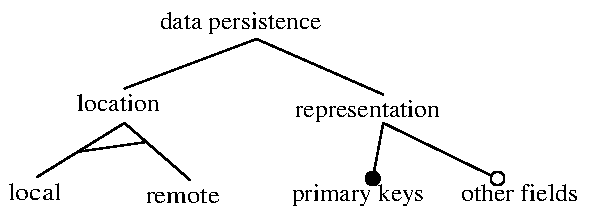
\includegraphics[width=10cm,height=!]{ch03/foda}
	\end{center}
	\caption{Feature Representation of Data Persistence}
	\label{c3fig:foda}
\end{figure}

The idea is to model the top features of a domain, that would be handled by an attribute-based container, by using single attributes. For example, a single attribute can be used to represent a top-level feature, such as the need to persist the data in a mobile application. A simplified (non-complete) feature model of data persistence is shown in \fig{c3fig:foda}. The data may need to be stored locally in the device, or remotely on the server-side. The possible representation model of the data needs to be decided for each component, e.g., to identify the fields that will serve as primary keys. Similarly to a feature model, attributes can be grouped in tree-like name spaces, where each name space is used to model different parameters of a single product-line asset. Sub-attributes are added as necessary to follow the feature model, and obtain a tree-like view of the modeled domain concerns. Attribute name spaces will be called \textit{attribute families}, and a C++ \cite{cpp.97} namespace-like dot notation will be used to organize them. The parameterization of attribute families is done by using nested attributes, or attribute parameters.

\begin{figure}[ht]
\begin{minipage}[t]{0.5\linewidth}
\begin{center}
\begin{scriptsize}
\begin{lstlisting}[numbers=left,language=Java,frame=leftline]{}
[dp]
[validate]
[property]
public class GameScore {

  [dp.pk]
  [dp.pk.sort("asc")]
  [validate.min(0)]
  [validate.max(100)]
  [property.accessor]
  private int score;

  [dp.pk]
  [dp.pk.sort("asc")]
  [validate.min(4)]
  [validate.max(32)]
  [property.both]
  private String playerName;

  [property.both]
  private String Comment;
}
\end{lstlisting}
\vspace{1.75cm}
\end{scriptsize}
\end{center}
\caption{Input Code}
\label{fig:input}
\end{minipage}%
\begin{minipage}[t]{0.5\linewidth}
\begin{center}
\begin{scriptsize}
	\begin{lstlisting}[numbers=left,language=Java,frame=leftline]{}
public class GameScore {
  private int score;
  private String playerName;
  private String Comment;

  public getScore() { return score; }
	
  public String setPlayerName(
    string value)
  { playerName = value; }
	
  // ...
  public byte[] toRecord()
  {
    ByteArrayOutputStream baos =
        new ByteArrayOutputStream();
    DataOutputStream outputStream =
        new DataOutputStream(baos);
    outputStream.writeInt(o.getScore());
    outputStream.writeUTF(
        o.getPlayerName());
    outputStream.writeUTF(
        o.getComment());
    return baos.toByteArray();
  }
  // ...
}
\end{lstlisting}
\end{scriptsize}
\end{center}
\caption{Output Code}
\label{fig:output}
\end{minipage}
\end{figure}

For example, consider the attribute-based implementation example of a \textit{GameScore} component in a mobile application\footnote{The example is based on the standard \textit{GameScore} example which comes with J2ME MIDP 2.0 \cite{www.midp-ota} documentation, explained in \kr{ch05}. The examples of  \fig{fig:input} and  \fig{fig:output} will be reused in \kr{ch04} to explain attribute-driven transformations.}, shown in \fig{fig:input}. The code in \fig{fig:input} is a declarative specification of the functionality encoded in \fig{fig:output}\footnote{The code in \fig{fig:output} is one possible result of mapping the code in \fig{fig:input} to a concrete implementation for a concrete mobile device.}. The fields in \fig{fig:input} are decorated with explicit attributes in the form of special \texttt{'[]'} comments. The following attribute families correspond to the different generic domain assets \see{c2.container.domain} that have been used in the code of \fig{fig:input}:
\begin{itemize}
\item \texttt{[property]} - adds accessor / mutator methods for a field (lines 3, 10, 17, and 20).
\item \texttt{[validate]} - adds validation code for fields that have mutator methods; \textit{min, max} show the required range for an integer or the required length ranges for a string field (lines 2, 8, 9, 15, and 16).
\item \texttt{[dp]} - adds data persistence methods to the component, and enables retrieving the data records sorted based on the primary keys (presented as an attribute sub-family \texttt{dp.pk}) (lines 1, 6, 7, 13, and 14).
\end{itemize}

The organization of attribute families is similar to organizing other language abstractions into name spaces and enables the reuse of attribute names with overloaded semantics, reducing the total required vocabulary. For example, all attributes related to the persistence of data in a device start with the \texttt{db} prefix (lines 1, 6, 7, 13, and 14 of \fig{fig:input}). Attribute parameters, e.g., \texttt{"asc"} in line 7 of \fig{fig:input}, are used to support the variability of the specific attributes inside an attribute family. Attribute families provide a convenient method to organize the domain functionality. All domain assets are organized as a tree of attribute families. Similar to language name spaces, attribute families can contain nested sub-families that group the variability of similar concepts, e.g., \texttt{db.pk}, groups the variability parameters related to the primary keys (lines 6, 7, 13, and 14 of \fig{fig:input}).

Based on the domain features, the architectural space of a product-line can be designed and its programming model can be decided. In \cite{generative.00}, the domain features are divided in four classes: concrete, aspectual, abstract, and grouping. As explained in section \see{c2.container.domain}, the container-based view of a product-line enables a uniform treatment of generic and specific assets and their features. The programming model can be represented by attribute families. Attributes enable a uniform representation of all the feature groups distinguished in \cite{generative.00}. For example, the concrete implementation of the data persistence feature of \fig{c3fig:foda} will be a \textit{concrete} component as part of the product-line services. The instantiation of the data persistence feature is, however, \textit{aspectual}. The specification of the primary keys needs to refer to a particular component implementation. Attributes connect the feature-based variability, implemented as part of the product-line services, with the fine-grained feature variability code written manually by the developers.

Ideally, attribute families enable the presentation of the domain features declaratively, without giving any clues about the implementation details of a given feature. In practice, the level of abstraction modeled by an attribute family is as good as the feature model used to create it. Attribute can also quickly reflect the evolution of a feature model. As explained in section \see{sec:gaast}, attribute-enabled languages offer a lightweight mechanism to support the evolution of the declarative constructs in code. 

\subsection{Attribute Parameters}
\label{ch03:sec:attrib.param}

Attribute parameters are a convenient mechanism to specify the domain variability, modeled by using attributes. This section discusses how attribute parameters can be included formally in the overall attribute model. The discussion hitherto has assumed that attributes have the following EBNF \cite{Parsing.Techniques.90} form: {\tt attributeName :=\- (paramterName =\- pa\-ra\-me\-terVa\-lue)*}. An attribute is identified by a name and by any (optional) parameters that it takes.

A distinction can be done between \textit{structural} attribute parameters that are known at compile time (usually static constants), and \textit{behavioral} parameters whose value can be determined (dynamically) only at run-time. When attributes are used for generation, they can contain only compile time evaluated parameters. Run-time evaluated parameters usually need some form of run-time support. Behavioral parameters are similar to introducing additional method / constructor arguments, and can be handled as such in the systems that need them.

When speaking about attributes, their structural parameters will be implied without making any special assumptions about them. Using parameters is only a convenience in using tags for annotations. While parameters help to express attribute variability more declaratively, they do not make annotations more powerful as summarized formally by the following theorem:

\begin{theorem}
\label{theo:tagParam}
Tags with explicit structural parameters can be always replaced with tags without parameters in a given program.
\end{theorem}

\noindent Proof: Let T be a tag and $\pi$ its parameters vector. It should be proved that (i) there exists a discrete function F: (T, $\pi$) $\to$ T', that returns a new tag T' based on the tag T and its parameters $\pi$ and (ii) that F is a finite function, that is, it has a finite co-domain. Indeed:\\
(i) Let F: (T, $\pi$) $\to$ T' be a function constructed by expressing all the parameters $\{\pi\}$ as strings that are joined together with some string separator (e.g: '\$'), and appended to the tag T, for example T' = T\$$\pi$. The function F returns a unique tag for any tuple (T, $\pi$). If '\$' is escaped inside T and $\pi$, then F has also an inverse function F$^{-1}$: T' $\to$ (T, $\pi$).\\
(ii) The function F is a total function over $\{\pi\}$. If $\{\pi\}$ is an infinite set then so is F. But the number of structural elements in a given program is finite. Thus, even though $\pi$ could be infinite, only a finite set of its values are used in a given program. So, F can be replaced with a finite set of partial functions over $\pi$ (QED).

\subsection{Connecting Attribute DSA with Product-Line Assets}
\label{dsa.connect}

Representing DSA with attributes in code removes the costs related to the grammar modification. Attribute-based DSA should, however, be interpreted and properly connected to product-line services. For example, the code in \fig{fig:inject} shows the attribute-decorated \texttt{Ga\-me\-Score} class of \fig{fig:input}. The used attributes state that the \texttt{Ga\-me\-Score} objects should be made persistent in the memory of a mobile device. The persistence requirement is expressed declaratively as a set of attributes, e.g., \texttt{dp}\footnote{Data Persistence Object.} in the \texttt{Ga\-me\-Score} class definition.

\begin{figure}[ht]
	\begin{center}
		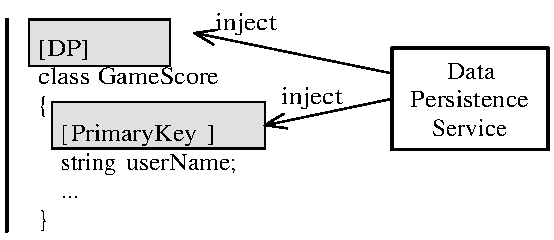
\includegraphics[width=8cm,height=!]{ch02/inject}
	\end{center}
	\caption{Connecting Attributes with Services}
	\label{fig:inject}
\end{figure}

The declarative attribute-based DSA notation needs to be connected to the actual data persistence code (service). The connection can be implemented in a variety of ways, for example by enhancing the compiler to detect and process the attributes, or by using some other way to organize services, such as, as component libraries or templates, and then bind them to the attribute-decorated code as required. Given that the focus is on easy to implement and to maintain DSA mechanisms, extending the compiler is not an option.

\Sr{c2sec:containers} already discussed how product-line assets can be organized as services that are transparently managed by a software container abstraction. \Kr{ch04} develops a technology to implement modular attribute-based transformers, which helps to develop low-cost attribute-based DSA transformations and connect them to the product-line services. Attributes can be interpreted before, or after compilation, or at runtime. Attribute interpretation requires to somehow be able to access and eventually modify / transform some AST-like source- or binary-level representation of the annotated program. For instance, tags used in MOF / UML can be interpreted when the model is transformed to another more detailed model. JavaDoc attributes used in Java 1.4 can be interpreted when the source code is processed. .NET attributes, or Java 1.5 annotations are saved as part of the binary meta-data. This enables the manipulation of binaries after compilation, or the run-time interpretation of tags by using the Reflection API. The run-time interpretation requires that the original annotated program is structured in such a way, that it can be compiled without interpreting the tag semantics. For example, in .NET a method body cannot use a variable that will be introduced by an attribute interpretation, because such a method cannot be compiled.

This chapter concentrates on language technology for supporting and facilitating the construction and maintenance of attribute-based DSA transformers. Before doing so, in order to complete the attribute-based software development (AESD) discussion, the advantages of AEP will be summarized, and ways to integrate attributes in the early phases of software development will be considered.

\section{Advantages of Attribute Programming}
\label{sec:gaast-mda}

This section compares the benefits of having access to explicit attribute support at the language level, with other techniques to model domain abstractions in source code, namely marking interfaces and pseudo-syntax marking. A typical model mapping scenario from \textit{Model-Driven Architecture} (MDA) \cite{mda,mda.frankel} is used. The goal of MDA is to increase the level of abstraction of software development. MDA enables software developers to specify "what" a software solution should provide, rather than "how" to realize the desired solution in terms of the technicalities of a particular implementation platform. The "what" is specified in a so-called \textit{Platform Independent Model} (PIM). Based on the chosen technology, there are different operations that can be used to realize a PIM, resulting in different \textit{platform specific models} (PSMs) of the same PIM. A PSM can be a ready-to-run implementation, or it may act as a lower-level PIM for further refinement to a new PSM that can be directly implemented.

Obviously, it is desirable to have an abstract PIM and to automate its translation to a given PSM implementation. A fully automatic transformation of any abstract model is not possible. Additional PSM specific directives need to be provided by applying marks from a specific profile\footnote{UML profiles modify the UML M2 model, i.e., they bring extensions to the M2 level.} to PIM elements. This implies a commitment to some kind of specific technology for solving the problem. The profile denotes the domain-specific notations, by using specialized forms of marking, e.g., tagged values and stereotypes. Marking represents concepts of the PSM in the PIM and indicates how the PIM elements are to be transformed \cite{mda.guide}. 

For illustration, \fig{fig.uml1} shows a simple web service with two methods, (i) to log in and authenticate a client (user) ({\tt Lo\-gin}), and (ii) to enable the client to access some user specific data ({\tt Access\-User\-Data}). The simple web service class, named \texttt{Web\-Ser\-vi\-ce1}, is modeled by the means of UML profiles. Three stereotypes {\tt \flqq web\-ser\-vi\-ce\frqq}, {\tt \flqq namespace\frqq} and {\tt \flqq uniqueid\frqq} are defined. The last two can also be represented as tagged values connected to the {\tt \flqq web\-ser\-vi\-ce\frqq{}} stereotype. In addition, two free tagged values, \texttt{ena\-ble\-Se\-ssion} of type \texttt{boolean} and \texttt{tran\-sac\-ti\-on\-Opti\-on} of type {\tt enu\-me\-ra\-tion}, are used to decorate the methods of this web service.

\begin{figure}[ht]
	\begin{center}
		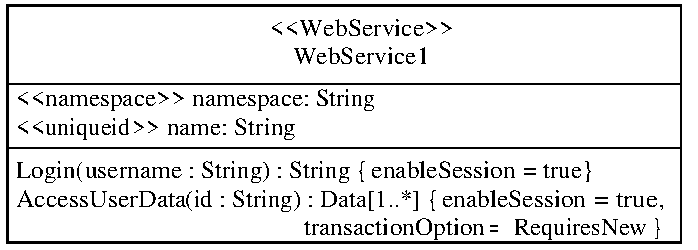
\includegraphics[width=8cm,height=!]{ch03/uml1}
	\end{center}
	\caption{Modeling using UML Profiles}
	\label{fig.uml1}
\end{figure}

Compared to a more abstract counterpart that does not contain any of the above tags, the model of \fig{fig.uml1} is technology dependent. Several technology commitments are made by using the profile. First, it is decided to expose the component as a web service. Second, the technical concerns needed by the service methods are explicitly enumerated, e.g., session and transaction management. However, at this point there is not yet any commitment made on how the session and transaction management will be implemented. The example only states the need for such technical services by means of the specialized UML profile, but has not yet committed to a particular web service platform.

In the MDA terms, the model in \fig{fig.uml1} is still a PIM for a more specific PSM. Given such a marked PIM, some transformer \texttt{T$_{1}$} is applied to produce a lower-level PSM, as shown schematically in \fig{fig.mda-model}. In MDA the commitment about the technology is done in stages rather than at once. The rationale behind this stratified commitment \cite{kuhne.01} is that a model of a higher-level stage can be mapped to more than one possible model of a lower stage. A staged commitment makes it possible to exchange the lower-level models, while preserving the investment on the higher-level models.

\begin{figure}[ht]
	\begin{center}
		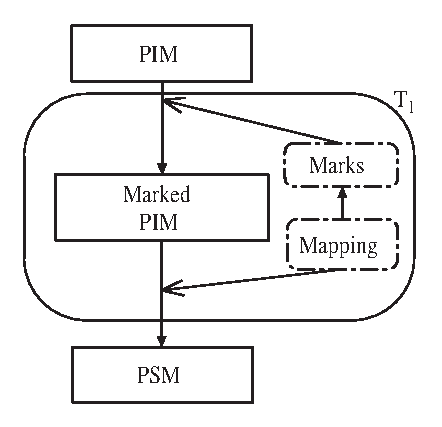
\includegraphics[width=4.5cm,height=!]{ch03/mda-model-orig}
	\end{center}
	\caption{MDA PIM-to-PSM Transformations}
	\label{fig.mda-model}
\end{figure}

Assuming that the target PSM is expressed in a programming language, the transformer \texttt{T$_{1}$} knows (a) how to map marks to corresponding language constructs, and (b) how to map types used in the model, to types of the target programming language, e.g., a \textit{String} in the modeling language may map to a character array in the target programming language. Type mapping is usually easy to handle automatically and will be not addressed any further. By selecting a given language, a further commitment is made on what the final software will be like. Selecting the target language says still nothing about how issues, such as sessions and transactions, will be implemented by tag interpretation (eventually in a later stage). Concerning the tag mapping, in the case when the target PSM (\fig{fig.mda-model}) is expressed in a concrete programming language, it could be distinguished between:
\begin{itemize}
\item mapping the tags to language constructs, and 
\item interpreting the language constructs to insert the specific concern's functionality.
\end{itemize}
  
A specific transformer may combine all three stages (mapping types, mapping marks to language constructs, and interpreting the latter) into a single pass. For instance, in addition to type and tag mapping, \texttt{T$_{1}$} (\fig{fig.mda-model}) may also interpret the tags. In this case, \texttt{T$_{1}$} commits to concrete session and transaction implementations and produces an executable PSM.

However, it makes sense to separate tag mapping from tag interpretation, when the transformation of a  PIM to an executable PSM is not fully automatic. This is the case when modeling is used only for defining the high-level architecture of an application. For example, in an EJB \cite{www.ejb} application, it is preferred to model beans and their interactions by means of UML constructs. It is easier to write and maintain complex business functionality directly in Java rather than to model {\tt for} loops and similar constructs using the UML action language \cite{www.uml}\footnote{The UML action language might be well suited to model embedded systems, where full automation of the transformation would make sense.}. In the web service example, issues, such as sessions and transactions, will be handled automatically. Programmers may still fill-in manually the functionality for logging and retrieving data by implementing the methods {\tt Login} and {\tt AccessUserData}.

As the focus is on programming language support for tag mapping and interpretation, the interest will be in lightweight mappings of tags to language constructs that do not require domain-specific additions to the target language. Such mappings are preferable because of lower costs for mapping arbitrary custom profile elements to a general-purpose language. The remaining of this section compares three widely used approaches for handling the mapping of tags to programming language constructs and for the interpretation of language constructs, namely: \textit{marking interfaces}, \textit{pseudo-syntactic marking} and \textit{attribute mapping}\footnote{A given tool may use any combination of these approaches.}. The comparison is done along the following dimensions:

\begin{enumerate}
\item \textit{Preservation of the PIM.} Preserving the architecture of the marked PIM in the source PSM is important, because it helps (a) to reverse engineer the source code PSM and (b) to understand the original PIM architecture by looking at source code alone. \fig{fig.text.1} shows an equivalent textual model of the web service of \fig{fig.uml1} in an extended\footnote{The introduced extensions address modeling profile elements. The current version of HUTN specification does not address any extension mechanisms for HUTN in order to keep the language simple \cite{hutn.dipl}.} HUTN\footnote{Human-Usable Textual Notation.} notation \cite{hutn}. The OMG HUTN standard is aimed at defining textual equivalents of MOF / UML diagrams which can automatically be generated. The tags of the web service example are modeled as extended adjectives in terms of HUTN. It is desirable that the source code PSM preserves the PIM structure to the same degree as the HUTN representation.

\begin{figure}[ht]
	\begin{center}
	\begin{minipage}[t]{8cm}
		\begin{scriptsize}
		\begin{lstlisting}[numbers=left,frame=leftline,showstringspaces=false]{}
webservice "WebService1"
{
  namespace namespace : "www.st.tu-darmstadt.de"
  uniquieid name : "Simple Service"

  enableSession Login(username : String) : String
  enableSession transactionOption.RequiresNew
    AccessUserData(id : String) : Data[1..*]
}		
\end{lstlisting}
		\end{scriptsize}
		\end{minipage}
	\end{center}
	\caption{Extended HUTN Model}
	\label{fig.text.1}
\end{figure}

\item \textit{Complexity of the Programming Model.} As already mentioned, parts of the code need often to be filled-in manually by the programmer in the generated PSM code. The structure of the PSM produced by tag mapping directly affects how the programmer interacts with such code. It is preferable to keep the programming model simple.

\item \textit{Interpretation of Mappings.} Interpretation is the next step after marks are mapped into language entities. Different kinds of mappings result in different techniques of interpretation. The interest will be in how easy it is to interpret language constructs resulting from tag mapping by considering the native support that the language technology offers for this purpose.

\item \textit{Extensibility of the Profile.} Extending a profile is often a requirement rather than an option. It is preferable to have means which facilitate the introduction of custom extensions to profiles. To illustrate the discussion, suppose that a new traceability tag named { \tt log} is added to the custom web service profile of \fig{fig.uml1}. This tag, when used with a method, will generate code that logs all method invocations. In the discussion that follows, the tag will be added to the { \tt Login} method. Logging enables to register which users used the service, at what time, and which users failed to authenticate.
\end{enumerate}

\subsection{Mapping Marked PIMs to Marking Interfaces}
\label{attributes}

To implement mapping of the PIM of \fig{fig.uml1} in Java 1.4, interfaces are often used as a means to emulate marking code elements at the language level \cite{design.attrib,mda.frankel}. When the PIM of \fig{fig.uml1} needs to be implemented in Java 1.4, it could map to the Java model consisting of the classes and interfaces of \fig{fig.uml.2}.

\begin{figure}[ht]
	\begin{center}
		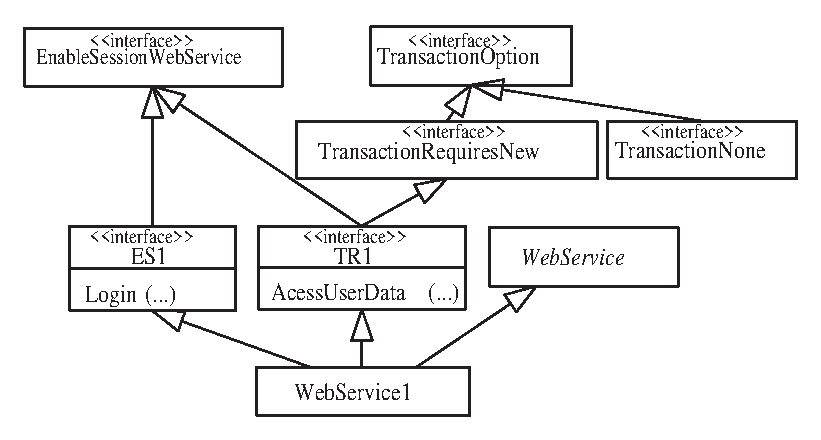
\includegraphics[width=10cm,height=!]{ch03/uml2}
	\end{center}
	\caption{Mapping by Means of Marking Interfaces}
	\label{fig.uml.2}
\end{figure}

For each tag and stereotype in \fig{fig.uml1}, a marking interface is introduced in \fig{fig.uml.2}. Multiple-value attributes are modeled as specialized interfaces that derive from other base marking interfaces. For example, \fig{fig.uml.2} assumes that the multi-value tag {\tt tran\-sactionOpti\-on} can only have two possible values, {\tt RequiresNew} and {\tt None}, which are modeled as children interfaces of the {\tt Tran\-sactionOpti\-on}. The stereotypes can also be modeled as marking interfaces, or as specialized (prototype) classes, e.g., {\tt WebSer\-vice} in \fig{fig.uml.2}. The mappings for the {\tt \flqq namespace\frqq} and {\tt \flqq uniqueid\frqq} stereotypes are not shown in \fig{fig.uml.2} and it is assumed that they are used in the implementation of {\tt WebService}. 

To emulate the tags of a given PIM method in a given class, a specialized interface for that method needs to be created. The specialized method interface derives from the basic interfaces that model the respective tags. For example, the interface {\tt ES1} inherits from {\tt Ena\-bleSe\-ssionWebSer\-vi\-ce} to make explicit that the method {\tt Login} is marked by the tag emulated by the {\tt Ena\-bleSessi\-onWebSer\-vice} interface. In the same way, the interface {\tt TR1} containing the method {\tt AccessUserData} is derived from {\tt EnableSessionWebService} and {\tt Tran\-sa\-ctionRe\-quires\-New} to reflect the fact that this method is marked by both {\tt ena\-bleSe\-ssion} and {\tt tran\-sac\-tionOption=Re\-quire\-sNew} in \fig{fig.uml1}. This way, the attributes of a method can be found by looking at the interface it belongs to.

\noindent Discussion:
\begin{enumerate}
\item \textit{Preservation of the PIM} - The mapping of \fig{fig.uml.2} does not preserve the modular structure of the PIM in \fig{fig.uml1}. From the model in \fig{fig.uml.2}, it is hard to guess the clear and concise structure and semantics expressed by the original PIM. The corresponding PSM code contains an explosive number of marking interfaces. This makes the PSM model more difficult to understand and hinders reverse engineering to the original PIM. The corresponding Java code of the UML model of \fig{fig.uml.2} will also be much more verbose compared with the textual HUTN representation of \fig{fig.text.1}. 

\item \textit{Complexity of the Programming Model} - Even though the example is extremely simple and several simplifying assumptions were done, the resulting PSM (\fig{fig.uml.2}) gets complex and verbose. Cross-interfaces need to be introduced, which inherit from base ones. The resulting PSM already mixes the business logic model with the model for implementing technical concerns. The technical concerns crosscut the modular structure of the business logic in \fig{fig.uml.2} and dictate the inheritance structure of the resulting program. The developer responsible for implementing the PSM in \fig{fig.uml.2} cannot "escape" some issues related to the implementation of the technical concerns. The developer has to know that interfaces, such as {\tt ES1}, exist and will be handled by a suitable concern automation environment.

\item \textit{Interpretation of Mappings} - Marking interfaces are not easy to interpret. Extracting the tags of a given method requires finding the interface where the method is declared, and retrieving the interfaces from which this interface inherits. When the interpretation is done at the source-code level, the full inheritance hierarchy must be resolved. Using compiled pseudo-binaries that contain meta-data, e.g., Java bytecode along with the Reflection API, makes it easier to resolve marking. Reflection relies on the existing virtual machine mechanisms to resolve the inheritance hierarchy. In order to extract knowledge about the marking interfaces hierarchy, the transformer that performs the mapping of marks must know the meta-model abstractions of the marked PIM. 

The overhead of tag extraction in terms of both complexity and performance of the interpretation logic cannot be avoided because the mapping of model tags to programming language constructs does not preserve tags as first-class values. First, as indicated above, the transformer that maps tags to language constructs is complex and needs to know the tag meta-model of the marked PIM. Second, the tag interpretation transformer needs to basically "undo" this work in order to extract tags from the marking interfaces resulting in a double overhead.

\item \textit{Extensibility} - To add a new {\tt log} tag to the method {\tt Login}, a new additional interface {\tt Log} need to be created in the language representation. In addition, the {\tt ES1} interface needs to be modified so that the web service class inherits from the new interface, in order to make explicit which new attributes the {\tt Login} method has. If {\tt log} were to be added to the other methods, the other interfaces need to be modified in a similar way. This would make the PSM model even more complex. Hence, the marking interfaces approach does not scale well. 
\end{enumerate}

\subsection{Mapping Marked PIMs to Pseudo-Syntactic Elements}
\label{ch03.pseudo.syn}

One way to decrease the number of the resulting marking interfaces is to rely on coding conventions, such as those used  in JavaBeans \cite{javabeans}, J2EE EJB \cite{www.j2ee}, or COMPOST \cite{java.compost}. Pseudo-syntactic marking uses string prefixes / suffixes to decorate the names of the marked elements according to some accepted convention based on the marked PIM. This approach will be called \textit{pseudo-syntactic marking}, because it adds new syntax to a language without really adding new keywords. 

Some systems, e.g., COMPOST \cite{java.compost}, rely on pseudo-syntactic marking for expressing class and member annotations. Other systems, e.g., JavaBeans \cite{javabeans} and J2EE EJB \cite{www.j2ee}, use a mixture of marking interfaces, required coding conventions, and annotations defined in so-called bean info objects (in the XML deployment descriptor). J2EE EJB implements class-level annotations by means of predefined classes / interfaces from which the annotated classes inherit. For methods and attributes, JavaBeans and J2EE EJB use pseudo-syntactic marking.
 
\begin{figure}[ht]
\begin{center}
\begin{minipage}[t]{8cm}
	\begin{scriptsize}
\begin{lstlisting}[numbers=left,language=Java,frame=leftline]{}
WebService1 implements WebService {
   String sessionLogin(String username) { ... }
   Data[] session_transactionAccessUserName(String id) {
     Transaction t = 
       context.getTransactionFactory().NewTransaction();
 	    ...
   }
}
\end{lstlisting}
	\end{scriptsize}
	\end{minipage}
\end{center}
	\caption{Using Pseudo-Syntactic Marking}
	\label{fig.pseudo-marking}
\end{figure}

For illustration, \fig{fig.pseudo-marking} shows how the web service of \fig{fig.uml1} could be mapped with pseudo-syntactic marking.
The {\tt \flqq Web\-Ser\-vi\-ce\frqq} stereotype is mapped to the predefined class {\tt WebService}, from which {\tt Web\-Ser\-vi\-ce1} inherits\footnote{A pure pseudo-syntactic marking approach would have used a \texttt{webservice\_} prefix.}. The \texttt{se\-ssion} and \texttt{se\-ssion\_tran\-sac\-tion} are used as required method name prefixes for methods {\tt Lo\-gin} and {\tt Access\-User\-Da\-ta} respectively. 
For analogy, in the EJB \cite{www.j2ee} model there are predefined types, such as {\tt SessionBean} or {\tt EntityBean}, as well as coding conventions, such as  \texttt{ejb\-Passi\-va\-te} or {\tt ejb\-Acti\-va\-te}.

\noindent Discussion:
\begin{enumerate}
\item \textit{Preservation of the PIM} - The original PIM is preserved better in this approach compared to the approach based on marking interfaces. 
However, pseudo-syntactic marking does not fully preserve the original PIM structure. Coding conventions and implementation restrictions imposed by a component model pollute the PSM, such that the details of original PIM get blurred. 

\item \textit{Complexity of the Programming Model} - Coding conventions for method prefixing reduce the exponential number of the emerging cross-derived marking interfaces. Compared to a PSM expressed by marking interfaces only, a PSM expressed by pseudo-syntactic marking hides some of the details for implementing technical concerns.  Pseudo-syntactic marking abstracts over the way the technical details are concretely realized by a certain framework model. The syntactic marks still need to be processed. Pseudo-syntactic marking also introduces new complexity at the programming model \cite{aspectComp.03}. The programmer has to be aware of the coding conventions and implementation restrictions encoded in the framework in use, which cannot be directly enforced by the compiler.

\item \textit{Interpretation of Mappings} - Pseudo-syntactic marking is more difficult to parse than marking interfaces because the transformer must use string operations on the code element names in order to extract tags. This can also cause performance overhead when done repetitively at run-time, due to the need for introspection. For example, a bean implementation in EJB needs to be introspected after it is compiled so that the container can generate and add glue code \cite{halloway.02}, e.g., to handle its passivation methods based on their name prefixes. 
As with marking interfaces, the overhead paid for tag extraction is introduced because tags were not preserved as first-class entities in the first place during mapping model tags to language constructs. No direct support is offered by the language technology for pseudo-syntactic mappings.

\item \textit{Extensibility} - Again, consider adding the new tag {\tt log}. The session concern can be represented as a new special prefix with pseudo-syntactic mapping, and the name of the method {\tt Login} will be {\tt log\_sessionLogin}. Such a schema is more fragile than marking interfaces because the new name could easily contradict with existing names, and may require a more careful code overview to avoid errors.
\end{enumerate}

\subsection{Mapping Marked PIMs to Attribute-Enabled Languages}
\label{sec.gaast.map}

As discussed in \sr{sec:gaast-mda}, the transformation of a marked PIM to a source code PSM can be staged into (a) mapping marking elements into language elements and (b) interpretation of such language elements. An attribute-enabled language helps with both (a) mapping marking elements to language constructs and (b) building transformers that do the interpretation. To deal with the issues present in other language representations, e.g., the preservation of PIM and the complexity of the programming model, a new element can be added to the MDA model of \fig{fig.mda-model}, represented by the gray box in \fig{fig.gaast-mda-model}. 

The transformer \texttt{T$_{2}$} performs the mapping of model tags to language level tags. 
The \texttt{T$_{2}$} mapping is straightforward, in the sense that tags are basically preserved and only written in a different syntax, since tags are first-class values in an attribute-enabled language. For illustration, \fig{fig.text.2} shows a possible mapping of the extended HUTN notation for the web service of \fig{fig.text.1} in .NET C\# language\footnote{The web service example was deliberately chosen to be a simplified version of the web service modeling semantics provided in the \texttt{System.Web.WebServices} .NET namespace.}. .NET C\# is considered an attribute-enabled language due to its explicit support for tagging in the form of attributes.
The attribute-driven transformer in \fig{fig.gaast-mda-model} is responsible for implementing the semantics of the tags. Compared to the interpretation of tags in the approaches discussed in the previous sections, the attribute-driven transformer does not need to do any tag extraction as attributes are full status elements. Implementing attribute-driven transformers is natively supported by attribute-enabled languages \see{sec:gaast}. 

\begin{figure}[ht]
	\begin{center}
		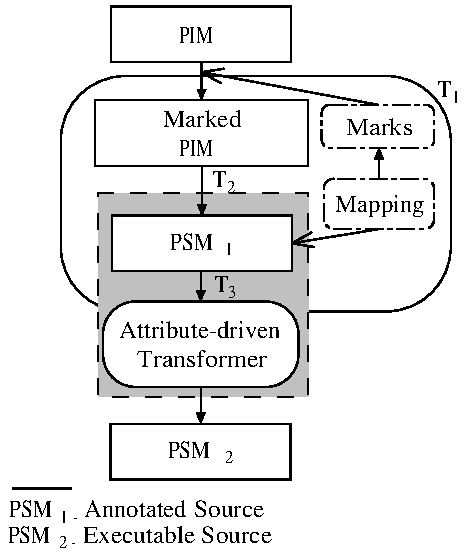
\includegraphics[width=6cm,height=!]{ch03/mda-model2}
	\end{center}
	\caption{MDA Attribute-enabled PIM-to-PSM Transformations}
	\label{fig.gaast-mda-model}
\end{figure}

%Let us now consider how the mapping and interpretation of marked models is different if the target language supports GAAST. 

\begin{figure}[ht]
	\begin{center}
	\begin{minipage}[t]{8cm}
	\begin{scriptsize}
\begin{lstlisting}[numbers=left,language=Java,frame=leftline,showstringspaces=false]{}
[WebService(namespace="www.st.tu-darmstadt.de",
  name="Simple Service")]
class WebService1 {
  [WebServiceMethod(enableSession)]
  string Login(string userName)
  {// TODO: add implementation code here}

  [WebServiceMethod(enableSession,
    transactionOption = TransactionOptions.RequiresNew)]
  ArrayList AcessUserData(string id)
  {// TODO: add implementation code here}
}
\end{lstlisting}
\end{scriptsize}
\end{minipage}	
	\end{center}
	\caption{Mapping to .NET C\#}
	\label{fig.text.2}
\end{figure}

\noindent Discussion:
\begin{enumerate}
\item \textit{Preservation of the PIM} - Converting the HUTN representation of \fig{fig.text.1} to C\# is straightforward. Apart from type and syntax mapping these models are actually equivalent. The transformer for the attribute mapping does not need to access the PIM meta-model. The transformer \texttt{T$_{2}$} can work at the M1 level. This is different from the case of transformers responsible for tag mapping in the marking interfaces approach. Marking interface transformers need details about the meta-model to do the transformation.

With the attribute representation, the model structure is preserved in source code, hence facilitating reverse engineering to the original PIM's architecture. The annotated source can sustain the full design architecture better than pseudo-syntactic marking without having to process method names, and without having to invent many method prefixes or suffixes. 

\item \textit{Complexity of the Programming Model} - The use of annotations simplifies the programming model because marks are still explicit. Having attribute-driven transformation support in the language framework provides the means for processing the language-level PIM. In other words, the part of the transformation concerned with introducing the details of "how" to realize the specified "what" is pushed entirely down to the language level.

The series of commitments in the MDA-based development could start by choosing the target attribute-enabled language. In an attribute-enabled language decorations based on attributes are used directly in code. This would be an alternative design to a graphical UML profile modeling step. Making programs look like designs improves the programming model, given that it decreases the intellectual gap to the domain concepts.

\item \textit{Interpretation of Mappings} -  The interpretation process in the marking interfaces and pseudo-syntactic marking approaches may require third-party tools which can parse and modify the input. An attribute-enabled language serves as a unified framework that does not require any additional third-party tools for parsing the input AST \see{sec:gaast}. 

Having the attribute processing be integral part of the language also simplifies the development of the transformers. Instead of relying on external systems to introduce custom parsing extensions to the language, the language is designed from the beginning to support such kind of transformations. The developer can focus on specific needs of the transformation, e.g., how to integrate transaction management, and not on the \textit{technicalities of the transformation itself}, e.g., on how to parse, access and modify the introduced linguistic abstractions for modeling transaction processing.

Shifting the transformation at the language level helps to achieve tool unification. The target development language is also the transformation tool. The transformation model supported by an attribute-enabled language is the only framework a developer must learn in order to deal with the transformation issues.

\item \textit{Extensibility} - Attribute-based mappings are modular because they directly preserve the PIM architecture and are easy to customize and extend. New issues can be dealt with at any time, by defining appropriate annotations and by introducing corresponding processors to the language framework. The {\tt log} tag example maps directly to a new attribute in this representation, and the mapping does not conflict with any of the other existing attributes. Nevertheless, still care is needed about the order of the transformation during the interpretation \seec{ch04}.
\end{enumerate}

\noindent This section concludes with a short discussion of some of the limitations of an attribute-enabled model-driven development (MDD): 
\begin{itemize}
\item Only the mapping of UML class diagrams with specialized profiles is directly supported by attribute-enabled languages. UML class diagrams map easily to an OO language. The attribute-enabled MDA process was illustrated by the means of the general-purpose object-oriented language C\# \cite{www.dotnet}, whose meta-model maps directly to the class-based web-service model. The transformation process may not be as easy when the UML model elements cannot be directly mapped to the target OO language. Other UML constructs cannot be mapped directly to the source code of a OO language. That is, attribute-enabled languages do not address the complete UML-based modeling of MDA.  %Besides, some profiles contain domain-specific tags that map to well-defined elements of some framework. This has to do with tag interpretation rather than with tag mapping to language constructs. 
%However, if no more specialized domain constructs exist for a given PIM, we could note that given that UML design is OO based \cite{Thomas.Uml.2003}, a general-purpose OO language with GAAST support, makes it easy to map any UML class diagram constructs to source level.

\item
The integrated attribute processing greatly facilitates, but does not automate the implementation of the transformers. While it enables the transformer programmer to concentrate on the semantics of the technical concerns to be integrated rather than be concerned with issues, such as tag extraction, the technical concerns semantics and interactions among transformers still need to be taken care of by the programmer. 
\item
Only the PIM structure is preserved in the language level PSM. Other more fine grained models of the method internals (e.g., using UML actions) will be lost, so only structural reverse engineering is possible. 
\item
The target language must have support for attribute-driven transformations.
\end{itemize}

%Our discussion in this section indicates that we are still away from such vendor supported language technologies that can fully support arbitrary and transparent transformation of source code or meta-data enabled binaries.

\section{Representing Explicit Attributes in {UML}}
\label{sec:problem-statement}

Attributes play an important role in representing custom design-related meta-data \cite{design.attrib,aop.attrib.05,www.aop.metadata,java.compost}, and can be used to expose joinpoints \cite{kiczalesetal.97} \see{ch2:aop}. These usages of attributes require an appropriate representation of attributes at the design time and therefore in UML  \cite{www.uml} diagrams. Several UML extensions using stereotype-like notations have been proposed to deal with specific joinpoints in OO class diagrams \cite{dong02,berner99,aspectj.uml.05}, but none of them deals directly with explicit attributes.

While attributes are similar to MDA MOF \cite{www.mof} tags and UML \cite{www.uml} tagged values or stereotypes, the effect of using attributes explicitly in a programming language, e.g., with Java 1.5 \cite{www.java.meta} annotations and .NET \cite{netattrib} attributes, opens new perspectives to design and program software. UML tagged values and stereotypes model only a subset of design possibilities that can be covered with explicit attributes. This section elaborates on the issue of representing attributes in UML, comparing different possible alternatives that can be used to model different design scenarios. The interest is to find convenient ways to represent explicit attributes in the UML class diagrams.

There are several issues with regard to representing attributes in UML. The first issue comes the used the terminology. In UML (and MOF) the term \textit{attribute} is used to denote class fields: in accordance with OO terminology, a class contains methods and \textit{attributes}. The term is also used with a generic meaning in the UML documentation, synonymously with the term \textit{property}. The term \textit{annotation} does not have any strict meaning in UML. It is used in the UML documentation mainly to denote text notes, i.e., comments. The best fit for a corresponding term for .NET \textit{attributes} and Java \textit{annotations} in UML (and MOF) are \textit{tagged values}. Tagged values are one of the three extensibility mechanisms available in UML (the two others being \textit{constraint} and \textit{stereotype}).

\begin{dinglist}{43}
\item \textit{A tagged value is a keyword-value pair that may be attached to
any kind of model element (including diagram elements as well as semantic
model elements). The keyword is called a tag. Each tag represents a particular
kind of property applicable to one or many kinds of model elements. Both the
tag and the value are encoded as strings. Tagged values are an extensibility
mechanism of UML permitting arbitrary information to be attached to models.}
(UML 1.5 Section 3.17.1 \cite{www.uml})
\end{dinglist}


The UML specification \cite{www.uml} defines in section 3.17, a standard notation for representing tagged values and other custom properties in class diagrams (which describe the static structure of the system). Properties of an element are written after all other data for that element have been specified.

\begin{dinglist}{43}
\item \textit{A property (either a meta-model attribute or a tagged value) is
    displayed as a comma delimited sequence of property specifications all
    inside a pair of braces ( \{ \} ). A property specification has the form
    name = value where name is the name of a property (meta-model attribute or
    arbitrary tag) and value is an arbitrary string that denotes its value. If
    the type of the property is Boolean, then the default value is true if the
    value is omitted.} (UML 1.5 Section 3.17.2 \cite{www.uml})
\end{dinglist}

\noindent There are, however, several problems with the property notation for modeling .NET attributes and Java annotations:

\begin{itemize}
\item Tagged values can only represent a single \textit{\textit{(key, value)}}
  pair. .NET attributes and Java annotations can take more than one
  \textit{(key, value)} parameter. For example, an
  \texttt{[Au\-thor]} attribute may require name and department parameters
  (e.g., \texttt{[Au\-thor(Na\-me=Va\-sian,\-De\-part\-ment\-=TUD)]}). The parameters can
  also be named or positional. Coding this information as a special escaped
  string, in the value part of a tag, makes it error-prone and difficult to
  parse.

\item In .NET, an attribute is a class, whereas in Java it is a special form of
  an interface. That is, a .NET attribute or a Java annotation exists as a
  separate class diagram element in a UML design. By representing an explicit
  attribute as a tagged value, it is impossible to distinguish between a tagged
  value and an attribute by looking at the notation only. A special notation can be used, e.g., an '@' prefix, for those keys that denote attribute names. However, this convention is not supported by default in the UML standard.

\item .NET attributes and Java annotations can take complex type values as
  parameters, such as arrays of constants, or other attributes. The UML tagged
  value notation can be become overloaded with all this information.

\item A .NET attribute and a Java annotation can be used to decorate not only a
  class but also inner class elements, e.g., fields, methods, method parameters, and the return type. The UML property notation can be used in all these cases, but the
  diagrams may become overloaded with information.

\item .NET attributes and Java annotations are used here to
  represent domain-specific abstractions. In this context, attributes serve as a kind of parametrized stereotype, and have the same weight in the design, as a stereotype. The property notation, which is specified after all the other information for an element, does not give any visible clue about the relative weight of the attributes in the design.

\end{itemize}

There is more than one possible alternative for presenting attributes in UML class diagrams\footnote{The issue of presenting
attribute definitions in UML will not be addressed, given that an attribute is similar to a stereotype. As attributes are first-class entities in Java and .NET, attribute definitions can be easily mapped to definitions of a specific
\flqq{}attribute\frqq{} stereotype notation, used to decorate attribute
classes in .NET and annotations interfaces in Java.}, with tagged values being the first candidate. The remainder of this section discusses several alternative UML presentations of explicit attributes, and presents criteria for analyzing the benefits and drawbacks of each notation accordingly.

\subsection{UML Alternatives for Explicit Attributes}
\label{sec:possibilities}

Several UML-based representations could be used to include
explicit attributes in class diagrams. While all these notations use UML
standard mechanisms, they all extend the UML notation in one or more ways.
The intention is to enumerate the most useful possibilities, and analyze the benefits and drawbacks of them. The different UML alternatives are compared based on the following criteria:

\begin{description}

\item[Standard Compatibility:] How good does the notation relate to the overall
  UML standard. Notations that are as near as possible to the UML standard are preferred. Related to standard compatibility is \textit{tool support} (integration in
  existing tools): Existing UML tools  \cite{case.tools} can easier support minor extensions that fit into the overall UML designs, rather than major changes.

\item[Visibility:] How good does the notation emphasize the importance of
  attributes in a UML design. Notations that emphasize the
  attribute semantics are preferred. Explicit attributes are often an
  important part of the design, and their relative weight should be properly
  expressed in the UML class diagrams.

\item[Clarity:] How clear or verbose the notation is. The less
  verbose notations are preferred. Verbose notations can be difficult to manage when they are used to decorate internal class elements, e.g., method parameters. Verbose notations could also result in cluttering of the UML diagram with too many elements.

\item[Usability:] How easy it is to use or reuse a given notation, e.g., being able to have a single definition of an attribute in a diagram and then reuse it via associations. Reuse is preferred, as it means less maintenance efforts. Related to reuse is \textit{ease of use}, that is how convenient a notation is to use, in order to model an explicit attribute.

\item [Representation Structure:] The preferred notations sustain a more structured attribute representation, compared to those that simply represent attributes as 
  strings. Structured notations are less error prone and easier to manipulate
  automatically.

\end{description}

\begin{figure}[ht]
	\centering
	\begin{minipage}[b]{8.5cm}
	\begin{center}	
		\begin{scriptsize}
\begin{lstlisting}[numbers=left,language=Java,frame=leftline,showstringspaces=false]{}
@Author(
    name="Vasian Cepa",
    name="Sven Kloppenburg")
@DAO
public class Account {
    
    @PrimaryKey
    private string accountID;
    
    ...

    @Transactional(kind=Required)
    public void credit(float amount)  { ... }

    @Transactional(kind=Required)
    public void debit(float amount)  { ... }
        
    public float getBalance() { ... }

    ...
}
\end{lstlisting}
		\end{scriptsize}
	\end{center}
	\caption{Attribute Annotation Example}
	\label{fig:app.example}
\end{minipage}	
\end{figure}

\noindent The main possible alternatives for presentation of
explicit attributes in the UML class diagrams are discussed next. The example of \fig{fig:app.example}, modified from \cite{www.aop.metadata}, will be used to illustrate the various alternatives.  The example shows how a bank account class can be modeled by utilizing several Java 1.5 annotations. There are two class level attributes: \texttt{[Author]} and \texttt{[DAO]}\footnote{Data Access Object.}, that denote the authors of the class, respectively, that the class needs to be processed in order to enable data persistence. Inside the \texttt{Account} class, there is a string field \texttt{accountID}, which is decorated with a \texttt{[PrimaryKey]} attribute as part of the data persistence functionality. This field will be used to identify the \texttt{Account} class records, when they are persisted in the database. Several of the class methods are decorated with a \texttt{[Transactional]} attribute, to denote that they must always be called as part of a transaction. Of course, not all code entities have attribute annotations, as illustrated by the \texttt{getBalance()} method. The UML examples below use a \textit{tilde} ('$\sim$') sign to separate multiples values in a UML property string value notation as needed, and an \textit{at} ('$@$') sign to decorate attribute name strings. Possible alternatives are separated with \textit{semicolons} ('$;$').

\begin{description}

\begin{figure}[ht]
		\centering
		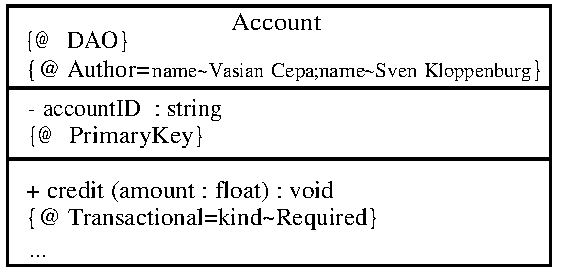
\includegraphics[width=7cm,height=!]{append1/properties}
	\caption{Attributes as UML Properties}
	\label{fig:tagged.values}
\end{figure}

\item[UML properties, tagged values:] This is the first UML representation possibility that comes to mind for attributes. The details and problems of this case were discussed in \sr{sec:problem-statement} to motivate the need to explore other notations. In order to represent the explicit attributes, the property notation needs to be extended (a) with a special notation, e.g., '@', used before the attribute names, and (b) to enable the string values to have an inner structure, in order to represent the key--value pairs of the attribute arguments. The extended notation is illustrated in \fig{fig:tagged.values}.
  
  The modification of the UML standard is minimal, and could be easily supported by
  any existing tool that supports UML properties and tagged values. The
  notation can become verbose, when too many attributes and attribute
  parameters are used in a class, or other inner elements, e.g., method parameters. The attribute annotations applied to an element cannot be reused. The annotation has to be copied and pasted around. This notation is not very structured, especially the value part of the string, and can be error prone.

\begin{figure}[ht]
		\centering
		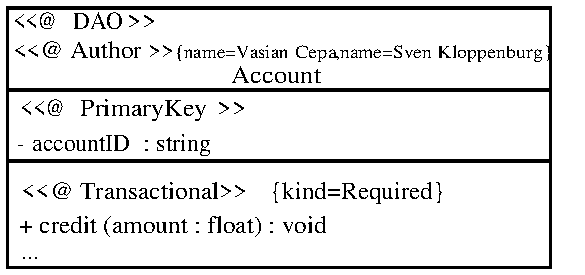
\includegraphics[width=7cm,height=!]{append1/stereotype}
	\caption{Attributes as UML Stereotypes}
	\label{fig:stereotype}
\end{figure}

\item[Stereotypes:] An alternative to the UML properties and tagged
  values for representing attributes is to use the stereotype notation, as in \fig{fig:stereotype} \cite{berner99}. In this case, the name of the attribute is used as a stereotype to decorate
  the UML elements. To distinguish a stereotype that serves as an attribute from other
  stereotypes, a special '@' character can be added before the name. An
  extension is needed to include the attribute parameter list with the help of a
  special notation, for example, by using an extended UML property notation as
  part of the stereotype instance name.

This notation is slightly better than the extended UML properties notation. Using the stereotype notation for the attribute name, rather than the usual property notation, shows explicitly the weight of the attribute in the design. It could also be relatively easily supported by the existing UML CASE tools. The notation is not very structured, especially the parameters part. 

\begin{figure}[ht]
		\centering
		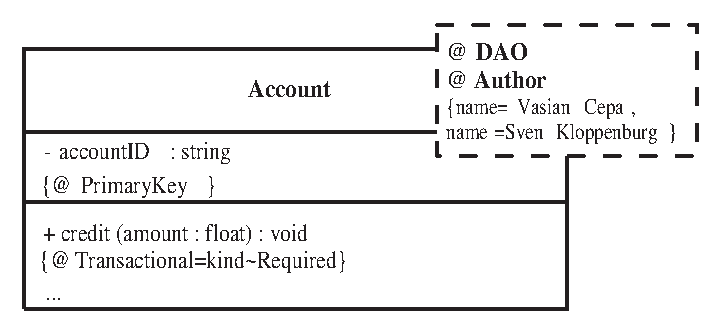
\includegraphics[width=9cm,height=!]{append1/template}
	\caption{Attributes as UML Template Parameters}
	\label{fig:template}
\end{figure}

\item[Template-like notation:] The C++ template argument notation,
  supported by the UML, can also be used to represent explicit attribute instances (\fig{fig:template}). This
  notation places even more weight to the role of an attribute, and could be
  useful in cases where attributes are very important in the design. The template notation can also be useful when the space inside the class-name box is scarce and there is a large number of attributes with a lot of parameters that need to be specified.
 
 The template
  notation will not work well with explicit attributes that annotate the inner
  elements of a class, e.g., object attributes, methods and method
  parameters. A variant of the template notation places in the template box the
  values of attributes for all member elements of a class, inside separate sub-boxes.
  This variation may require some kind of mapping between the
  attributes and the existing members. The notation could become verbose for
  the overloaded methods, where the method name is reused and cannot be used alone as a
  mapping tag. The template notation (without sub-boxes) could be easily supported by
  UML CASE tools. A benefit of the template notation is that all class-level attributes are located within a single easily visible place.

\begin{figure}[ht]
		\centering
		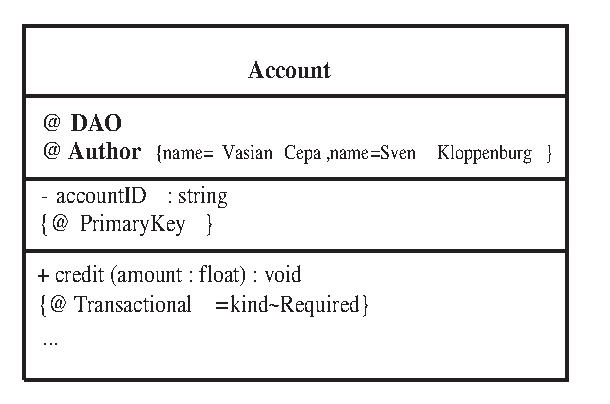
\includegraphics[width=7cm,height=!]{append1/box}
	\caption{Attributes as Extra Class Sub-Box}
	\label{fig:partition}
\end{figure}


\item[Class partitions:] Explicit attributes could form a separate sub-box inside the class notation, similar to
  fields and operations, as in \fig{fig:partition}.
  The sub-box notation could be seen as a natural way to extend the class
  definition semantics. Another variation is to have an explicit optional
  attribute sub-box for each kind of element in a class, such as fields and operations. The attribute sub-box is a stand-alone unit within the class model, and the notation has the same benefits and drawbacks of the template-like notation. The separate sub-box can be used in the UML tools that do not support the template notation.
  
\begin{figure}[ht]
		\centering
		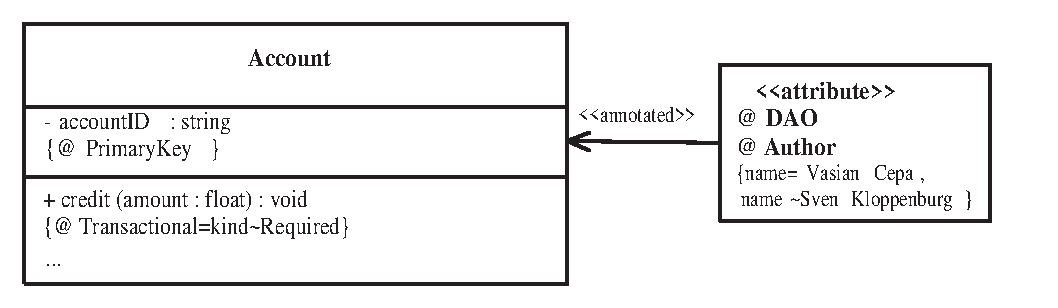
\includegraphics[width=12cm,height=!]{append1/class}
	\caption{Attributes as Separate UML Class}
	\label{fig:class}
\end{figure}

\item[Separate classes:] Explicit attributes can be also represented by a separate class-like notation with an \flqq{}attribute\frqq{} stereotype associated with the class, as illustrated in \fig{fig:class}. There are two variations of this representation: (a) one similar to the template notion, containing all the attribute notations for all
  elements of a class, (b) a separate class for the attributes of each inner element, associated directly with the annotated element.
  
  In the case of sub-elements, e.g., methods, the class notation may require that the association lines intersect the class boundaries and link directly to the methods or other inner elements, a feature that may not be supported by the standard conformant UML tools. The class notation is more reusable and more structured that the previous possibilities.

\begin{figure}[ht]
		\centering
		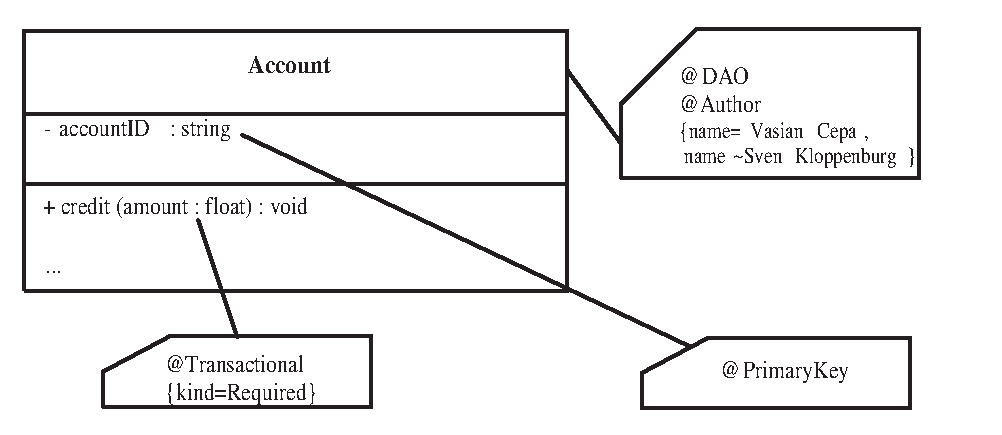
\includegraphics[width=12cm,height=!]{append1/comment}
	\caption{Attributes as Comment Boxes}
	\label{fig:comment}
\end{figure}


\item[UML comments:] Comments allow arbitrary text labels to be associated with every
  UML element. Comments can be used to model explicit attributes
  as shown in \fig{fig:comment}. Comments are unstructured, so there may be a need to place some implicit structure in the text string. For example, an '@' character can be used before a name to denote that it is an attribute.
  The selected implicit notation can be tool and language specific. The comment notation lacks the inner structure, and it may be difficult to distinguish between attribute comments and other types of comments in a diagram. Apart of this, the notation is as reusable and flexible as the separate class notation.

\end{description}

\subsection{Discussion of the UML Alternatives}

Table~\ref{tab:AttributePresentationInUML} summaries the above discussion, evaluating the alternative UML notations discussed above against the criteria given in \sr{sec:possibilities}. Plus signs indicate that a criteria is better supported. Minus signs indicate less conformance to a given criteria.

\begin{table}[ht]
	\begin{center}
		\begin{tabular}{|l||c|c|c|c|c|}
		\rowcolor[gray]{.7}
\hline
 Presentation &   Standard & Visibility &  Clarity &      Usability &  Structure \\

\hline
Properties &      + +      &      - -      &      - -      &      -      &      -      \\
\hline
Stereotype &       + +     &       +     &      -      &      -      &       -     \\
\hline
 Templates &       +     &       +     &       -     &       -     &      +      \\
\hline
 Partition &        -    &       +     &       -     &        -    &       +     \\
\hline
Separate Class &     +       &     + +       &     +       &     + +       &     + +       \\
\hline
   Comment &       +     &      +      &     -       &      + +      &      - -      \\
\hline
		\end{tabular}
	\end{center}

	\caption{Summary of Various Explicit Attribute Presentations in UML}
	\label{tab:AttributePresentationInUML}
\end{table}

As indicated by the Table~\ref{tab:AttributePresentationInUML}, no representation is better suited than all the other with regard to all criteria. The separate class notation seems to fulfill most of the requirements, however, it may have difficulties to represent the annotation of the inner class elements.

Table~\ref{tab:AttributePresentationInUML} shows that some notations are better suited that the others is some direction. This is a consequence of the various scenarios that could be covered with explicit attributes in a UML model. Depending on the
relative weight of the attributes in the design, their parameters, and the density of the attribute usage in a class, or in the class inner elements, different notations may be useful in different situations. 
%
For example, it could be chosen to represent attributes that serve as marking interfaces \cite{design.attrib} by stereotypes, given that this expresses their importance. When many explicit attributes are used to drive generation and they are repeated over classes, a separate class notation makes more sense. For fine grained notations, e.g., method annotations, or method parameter annotations, an extended variation of UML properties is less verbose and hence better suited. More than one notation could also be combined in the same diagram, as was the case with some of the UML examples in \sr{sec:possibilities}.

Finally, based on the Table~\ref{tab:AttributePresentationInUML}, it can be concluded
that the stereotype and separate class notations are the two most usable notations that should be considered as a first choice to model the explicit attributes in UML class diagrams. In several cases, some notation based on the UML properties is needed to augment the other representations. Several of the analyzed extensions may not be supported by all UML CASE tools.

\section{Languages with Generalized and Annotated Abstract Syntax Trees}
\label{sec:gaast}

This section discusses language technology organized around annotated Abstract Syntax Tree (AST)-like representations of program structure, used to support attribute-based DSA in product-lines. This section also discuses the impact of such technology on the processing of attribute annotated code entities.

%Generalized and Annotated Abstract Syntax Trees (GAAST) are a lightweight language extension mechanism relying on: (i) tagging program code with attributes and (ii) implementing transformations based on reflective-like Abstract Syntax Tree (AST) API-s. Two features are important for this purpose: (a) support for explicit meta-representation of programs as an AST-like structure accessible in a programmatic way before and beyond the compilation, and (b) support for user-defined annotations of program elements.

\subsection{Attribute Language Support Example: .NET Languages}
\label{c3.sec.dnet}

To illustrate the relation between annotations and AST-like representations of the program structure, this section considers .NET framework \cite{www.dotnet}, as a representative of systems with explicit support for tag interpretation, by means of access to source, or binary representations of programs.
%
.NET follows a hybrid approach with respect to attributes. It distinguishes between \emph{predefined} and \emph{custom} attributes. Predefined attributes are used by various library API-s that come bundled with the .NET platform. For example, \texttt{[Sy\-stem.Dia\-gno\-stics.Con\-ditional\-Attribute]} is used by the compiler to include methods conditionally in the compiled version. In contrast to the predefined attributes, custom attributes do not have a meaning to the compiler. The code to interpret custom attributes has to be implemented explicitly by the developer that introduces the attributes to model domain-specific concepts.

In .NET, an attribute is a normal class derived from a predefined \texttt{Sy\-stem.Attri\-bu\-te} class. Attributes are part of the type system and can also be marked with other attributes. The interpretation code can be placed inside the attribute class itself. When a larger context needs to be processed, in order to interpret the attributes, the interpretation code could also be placed in a separate module. 

\begin{figure}[ht]
	\begin{center}
		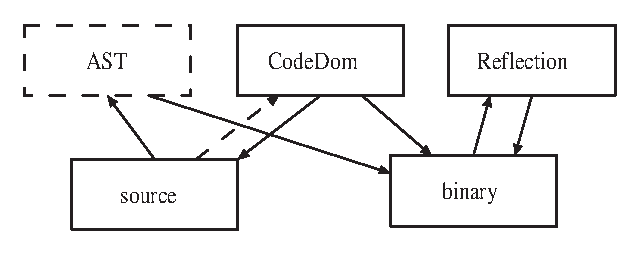
\includegraphics[width=7cm,height=!]{ch03/existing}
	\end{center}
	\caption{.NET AST-Like Program Representations}
	\label{fig.existing}
\end{figure}

\fig{fig.existing} shows a high-level view of the .NET API-s that support access to different AST-like representations of a program. There are by default two main ways how .NET API-s can be used to process attributes:

\begin{itemize}
\item \textit{Source code manipulation.} The .NET \texttt{Sy\-stem.\-CodeDom} API \cite{cdom}  supports source-level AST-like representation and manipulation of a program. An implementation of this API can be used to build an AST, either manually, or from the source code of a program (by means of \texttt{ICode\-Parser}\footnote{The current .NET framework language specific providers do not implement \texttt{ICode\-Parser}. For this reason, the connection from source to \texttt{CodeDom} box in \fig{fig.existing} is drawn as a dashed line. A free third-party implementation for C\# is \textit{CS CODEDOM Parser} \cite{cs.codedom.parser}.}). Next, the constructed AST-like representation can be transformed and the result AST is saved (back) as source (by means of \texttt{ICo\-deGene\-rator}), or it is directly compiled to a binary file (by means of \texttt{ICo\-deCompi\-ler}\footnote{ \texttt{Sy\-stem.Code\-Dom.Compi\-ler} interfaces (and helper classes) must be implemented by a \texttt{Code\-Dom} compiler provider.}).

\item \textit{Run-time manipulation.} The .NET {\tt Sy\-stem.Re\-fle\-ction} API can be used to (a) introspect a binary for its structural elements and the attributes they are decorated with, as well as in the reverse direction, (b) to create executable modules (assemblies). For the latter purpose the {\tt Sy\-stem.\-Refle\-ction.Emit} API can be used (in combination with the Reflection API) to generate the method internals. While the Reflection API deals with creating the program structure elements, e.g., classes and methods, the {\tt Emit} API deals with Intermediate Language (IL) opcodes used inside methods. The {\tt Emit} API works only in one direction. It can generate new assemblies, but cannot access or modify the IL representation of the existing ones.
\end{itemize}

\begin{figure}[ht]
	\begin{center}
		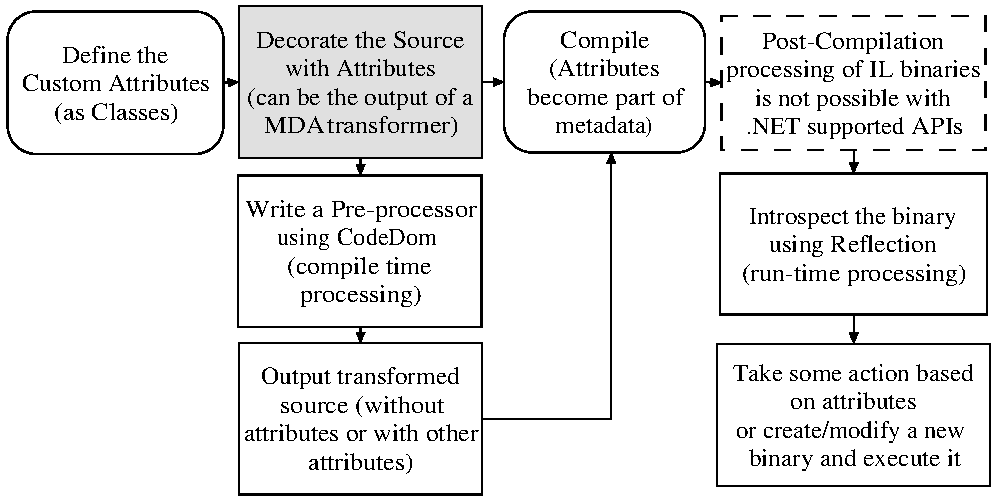
\includegraphics[width=12cm,height=!]{ch03/net-attribute-processing}
	\end{center}
	\caption{Processing Attributes in .NET}
	\label{fig.processing}
\end{figure}

.NET API-s provide an infrastructure for creating and accessing AST-like representations of a program beyond the parsing stage of the compiler. \fig{fig.processing} shows how this infrastructure can be used to interpret attributes in .NET. The first step to utilize the custom attributes in .NET consists in defining new attribute classes (when needed), and using them to decorate the code. The exact actions to be performed next depend on the semantics associated with the used attributes. In a next step, the source-level AST, obtained via  \texttt{CodeDom}, is used to modify the source code. Alternatively, the code is compiled and the attributes become part of IL binary meta-data. The IL meta-data are accessed later-on at run-time, via the {\tt Reflection} API, and are processed to undertake user-defined actions. Post-compilation manipulation of existing IL binaries is not directly supported by the .NET API-s.

\subsection{GAAST-Based Language Technology}
\label{sec.gaast}

\fig{fig.existing} contains also a dashed box named {\tt AST}, which is not discussed so far. This box represents the AST that is internally constructed by the compiler, during the compilation process of the source code. In .NET, this AST is not available to the end-programmers. The {\tt AST} box is shown in \fig{fig.existing} to emphasize the similarity between the different .NET AST-like representations of the program (aimed at supporting program transformations), and the source AST built by the compiler. The .NET CodeDom, or Reflection ASTs, and the compiler AST represent the same information at various levels of detail.

\begin{figure}[ht]
	\begin{center}
		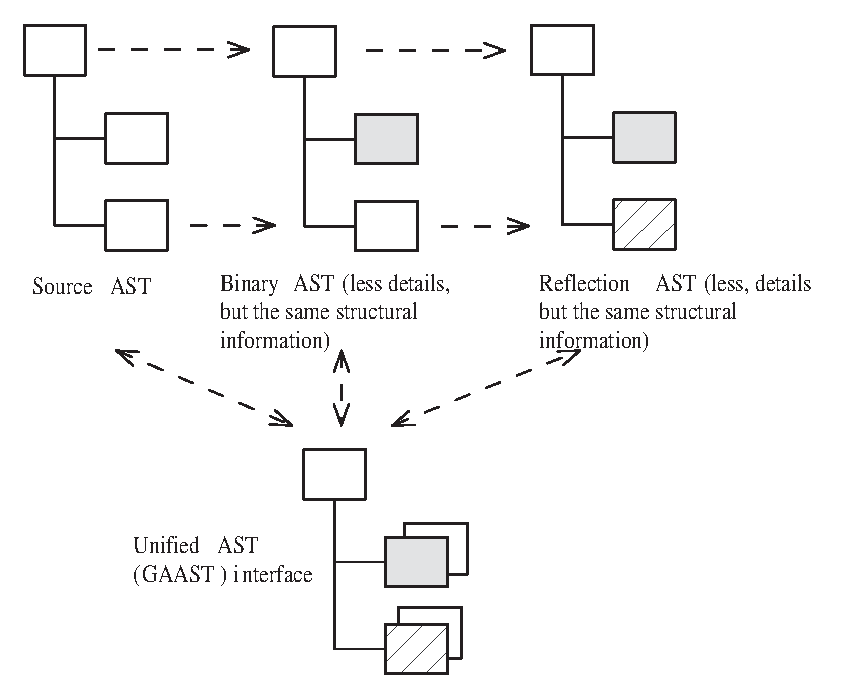
\includegraphics[width=10cm,height=!]{ch03/gaast}
	\end{center}
	\caption{Unified AST Representation}
	\label{fig.gaast}
\end{figure}

This similarity suggests the idea of having a single common AST-like representation of a program, that would be used by the compiler, as well as, by other attribute-driven transformers in a programming language with annotation support. Such an AST API, that generalizes over different ASTs of the same program and supports annotations, will be called a \textit{Generalized and Annotated AST} (GAAST) API. There are several aspects of a GAAST API that need to be especially discussed:

\begin{itemize}
\item \textit{Modeling AST differences.} As illustrated in \fig{fig.gaast}, there could be differences in the information found in different representations of the program. Some nodes present at source code are not preserved in the binary representation, or could be presented by different element nodes (gray filled in \fig{fig.gaast}). A common example is deploying a prefix or suffix increment / decrement operator. The GAAST API is intended to support attribute-driven transformation for implementing DSA constructs. The source code AST representation is too fine grained attribute-driven transformers. The GAAST API can unify the structural information and leave out the other details. Some nodes can be present in the interface, but a given implementation of GAAST may choose not fill all nodes with valid, or fully parsed information \see{dnet.gaast}. This situation is represented by different fillings of (possibly empty) nodes in the unified AST, at the bottom of the \fig{fig.gaast}.

\begin{figure}[ht]
	\begin{center}
		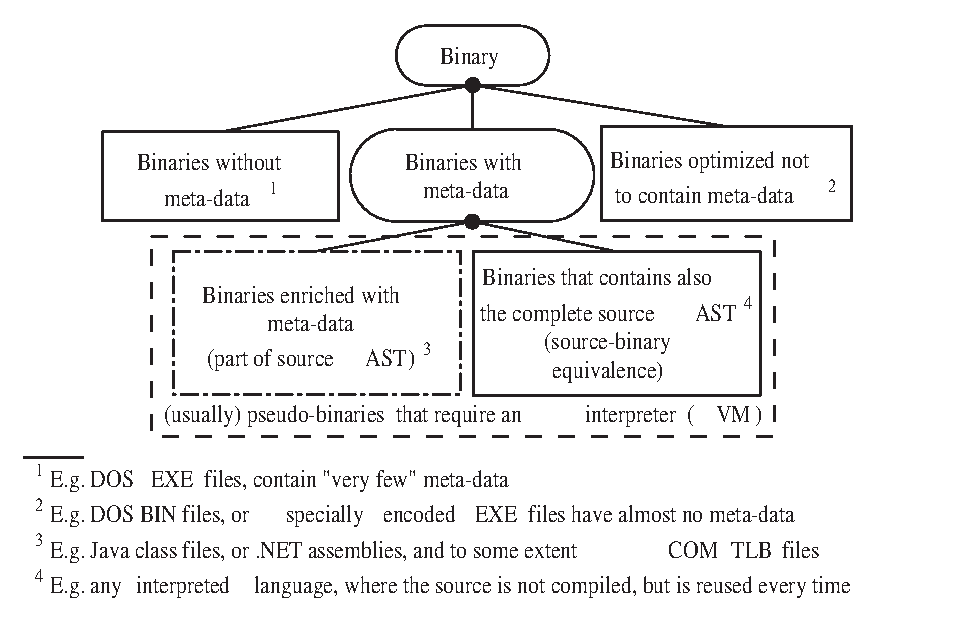
\includegraphics[width=12cm,height=!]{ch03/metadata}
	\end{center}
	\caption{GAAST Relation to Meta-data}
	\label{fig.meta-data}
\end{figure}

\item \textit{Matching the language features.} GAAST reflects the features and the dynamicity of the underlying language system. The source code manipulation enables static transformations. Many language systems support only static transformations, because they do not save the AST information as part of their \textit{pseudo-binaries}. \fig{fig.meta-data} shows a rough classification of what is understood by binaries in this section. The meta-data, as shown in \fig{fig.meta-data}, is a way to explicitly save part of the AST obtained from the source code along with the compiled code. The amount of the AST information saved as part of meta-data determines the level of reflection that is possible at run-time in a given language system. The reflective transformations require languages that have enough meta-data to support run-time introspection, represented by the dash-dotted box in \fig{fig.meta-data}.

Languages, such as Java or .NET, save almost all structural information found in source code as part of the binary meta-data. These language technologies usually do not preserve a one-to-one map of those parts of the AST that represent control-flow (behavior), e.g. \textit{for} loops. Obtaining such fine-grained control structures requires some reverse engineering. 
%
In languages that support meta-data as part of their binaries, the GAAST API could support also static binary manipulation. In reflective languages, GAAST may support either static or dynamic transformations, depending on the language run-time support for reflection.

\item \textit{GAAST as a Language Workbench.} Extending a programming language to support a GAAST-like API is relatively easily, when only specific features of GAAST are needed. For example, any static meta-programming framework can be used as a GAAST-like API for static source code transformations, as long as the framework preserves and enables access to the AST attributes. This makes a GAAST-like API an attractive lightweight language expression to support attribute-based transformations in mobile product-lines \seec{ch05}.

\begin{figure}[ht]
	\begin{center}
		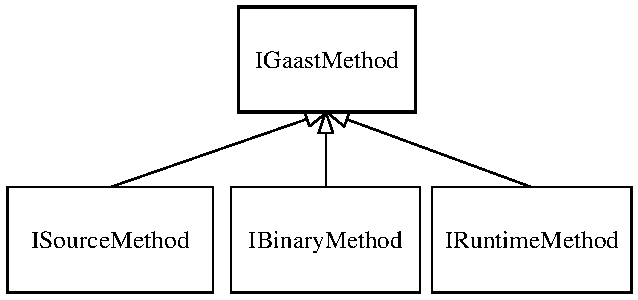
\includegraphics[width=6cm,height=!]{ch03/native}
	\end{center}
	\caption{GAAST Language Information Organization}
	\label{fig:native}
\end{figure}

A more advanced view is to consider GAAST as part of the language system itself. That is, to make the unified GAAST API a central part of a language framework supported by the language vendor. The other API-s, such as the compiler AST, {\tt Reflection}, or {\tt CodeDom}-like API-s, could be organized around the common GAAST interface, as illustrated by the method interface example in \fig{fig:native}.

A language with GAAST support for attribute-driven transformations can be seen as a language workbench \cite{lang.workbench} to sustain attribute-based DSA. The GAAST API serves as a \textit{contract interface} between the language workbench features, provided by the language vendor, and third-party attribute transformers. It becomes the responsibility of the language vendor to maintain the contract interface as the language evolves. Several languages, e.g., .NET or Java, are already moving into this direction.

In a GAAST-enabled language, the attribute transformers are immune to most changes in the language workbench (e.g., several syntax changes). This is difficult to warranty with third-party implementations that need to be separately maintained, adding accidental complexity to the product-line. In a GAAST-enabled language, the transformer developers would not need to reinvent helper API-s and tools that are covered by the GAAST API. Transformers could reuse third-party modules build on top of the central GAAST and better leverage rapid prototyping. The language platform vendors would also profit from the unified GAAST API, since by unifying several API-s, the total cost of the language platform is decreased and the language system becomes also more attractive to the programmers.

\end{itemize}

\noindent GAAST addresses only the parsing issues related to source or meta-data enriched binaries. Attribute-driven transformation based on GAAST-like API-s will be fully discussed in \kr{ch04}. Specialized abstractions could be built on the top of the GAAST API that would facilitate building transformers. There are two concepts that can be used in combination to implement generic abstractions over a GAAST infrastructure:

\begin{itemize}
\item GAAST can be enhanced with declarative query capabilities. An example of query capabilities is {\tt JPath} API for Java developed as part of {\tt EXTRACT} \cite{extract} compiler system. JPath defines a set of operations for selecting nodes from a Java AST, borrowing the idea from W3C XPath \cite{url.xpath} standard for XML \cite{skonnardetal.01}. Another example of query support directly embedded in the langauge, is the query expression pattern of .NET C\# 3.0 language specification \cite{csh30}, based on the LINQ \cite{linq} project.

\item Support for declarative specification of transformations. This is similar to the ideas put forward by OMG MOF Query / Views / Transformations (QVT) proposals \cite{mof.qvt}. In terms of QVT, JPath is a query and view language. QVT also exposes means to define transformations. Transformers take a view as a parameter and map it to another view. This is similar to graph rewriting techniques \cite{term.rewrite,mens.99,gme.graphs}, but provides a more declarative way to define graph transformations. At the time of this writing a final MOF QVT standard is not yet available. 
\end{itemize}

\subsection{Implementing GAAST on Top of .NET}
\label{dnet.gaast}
Having stressed the importance of supporting GAAST as a central part of the language technology, \fig{fig.third} shows how a third-party prototype GAAST API can be implemented on top of the existing .NET API-s.

\begin{figure}[ht]
	\begin{center}
		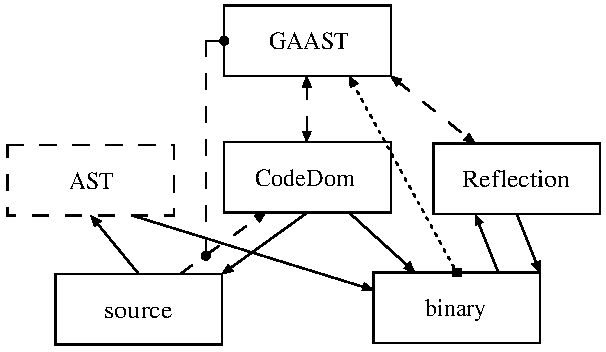
\includegraphics[width=7cm,height=!]{ch03/third}
	\end{center}
	\caption{Implementing GAAST on Top of .NET}
	\label{fig.third}
\end{figure}

The dotted arrow, from the {\tt binary} box to the {\tt GAAST} box, represents the required custom code to expose the method internals of IL binaries through the GAAST API, which is currently not supported by the .NET Re\-fle\-ction API. The dashed line connecting {\tt source} and {\tt Code\-Dom} boxes represents the implementation of the {\tt ICo\-de\-Par\-ser} interface, which is also currently missing in .NET.

Unfortunately, a third-party API cannot directly reuse the AST built by the language compiler(s), and does not have access to the .NET Common Language Runtime (CLR) information, unless a supported interface to expose this functionality is provided. The lack of this interface renders the implementation and maintenance of a third-party framework difficult, especially in face of the evolution of the .NET framework.

\begin{figure}[ht]
	\centering
	\begin{minipage}[b]{8.5cm}
	\begin{center}	
\begin{scriptsize}
		\begin{lstlisting}[numbers=left,language=Java,frame=leftline]{}
namespace System.Reflection {

 public class MethodInfo : MethodBase {
	
  public Type ReturnType
  { get{ ... } }
		
  public object[] GetCustomAttributes(bool inherit)
  { ... }
  ...
 }
}
		\end{lstlisting}
		\end{scriptsize}
	\end{center}
	\caption{Reflection API Method Representation}
	\label{c3:netref}
\end{minipage}	
\end{figure}

As an example, consider \fig{c3:netref}, that shows how the \textit{methods} information is modeled by the .NET Reflection API. The Reflection API enables the introspection of a method to get information about it, e.g., to find the custom attributes that have been used to annotate the method and its return type. When using the Reflection API, the types returned by the methods, e.g., \textit{Re\-turn\-Ty\-pe}, are properly resolved, and the system has access to the full loaded assemblies, which makes it possible to return, for example, the attributes inherited from a base class method (the \texttt{bool inherit} option of the \texttt{Get\-Cu\-stom\-Attri\-bu\-tes} method).

\begin{figure}[ht]
	\centering
	\begin{minipage}[b]{8.5cm}
	\begin{center}	
\begin{scriptsize}
		\begin{lstlisting}[numbers=left,language=Java,frame=leftline]{}
namescpace System.CodeDom {

 public class CodeMemberMethod : CodeTypeMember {

  public CodeTypeReference ReturnType
  { get{ ... } set{ ... } }
		
  public CodeAttributeDeclarationCollection CustomAttributes
  { get{ ... } set{ ... } }

  public CodeCommentStatementCollection Comments
  { get{ ... } }
  ...
 }
}
		\end{lstlisting}
		\end{scriptsize}
	\end{center}
	\caption{CodeDom API Method Representation}
	\label{c3:netdom}
\end{minipage}	
\end{figure}

\fig{c3:netdom} shows how the same information is modeled by the .NET Code\-Dom API. The first difference concerns the returned types. For example, the type returned by the \texttt{Re\-turn\-Ty\-pe} is not a fully-resolved \texttt{Ty\-pe}, but a \texttt{Co\-de\-Type\-Re\-fe\-rence}, which could be either an unresolved user defined type, or a resolved system type. Another difference is that the \texttt{Cu\-stom\-Attri\-butes} method cannot resolve hierarchy information. Information for additional nodes, e.g., code comments, is also present, which makes no sense for binary files. The most profound difference is the capability to modify the information, as can be noted by the \texttt{set} version of the supported properties in \fig{c3:netdom}. The Reflection API provides read-only access to the method information.

\begin{figure}[ht]
	\centering
	\begin{minipage}[b]{8.5cm}
	\begin{center}	
\begin{scriptsize}
		\begin{lstlisting}[numbers=left,language=Java,frame=leftline]{}
namescpace Gaast {
	
 public interface Method : Member {

  public Type[] ReturnType
  { get{ ... } set{ ... } }
		
  public CustomAttribute[] CustomAttributes
  { get{ ... } set{ ... } }

  public Comment[] Comments
  { get{ ... } set{ ... } }
  ...
 }
}
		\end{lstlisting}
		\end{scriptsize}
	\end{center}
	\caption{GAAST API Method Representation}
	\label{c3:netgaast}
\end{minipage}	
\end{figure}

A possible common GAAST-like interface is shown in \fig{c3:netgaast}. The GAAST interface enables writing the same structural transformations, despite the underlying program representation. When no complete native language support for GAAST exists, as is the case with .NET, a third-party GAAST API, based only on the CodeDom and the Reflection API, could only offer a set of uniform interfaces to access the common information. To initialize the GAAST interface, a factory pattern \cite{dpatterns} can be used, similarly to the way .NET CodeDom supports different .NET languages. The factory can support either source, or run-time representations. A trade-off to model the AST differences could be to ignore representation specific information and throw a missing implementation exception on \texttt{set} methods, when only a read-only view is supported.% The situation can be partially improved if other third-party frameworks for processing .NET binaries can be used and through custom access to the .NET CLR data, for example using the .NET profiler.

In practice, unless GAAST languages become available, a third-party GAAST API implementation can be reasonably limited, by implementing only those aspects of the GAAST technology that are needed by a specific transformation system. As the focus is on DSA support with attributes, only the static aspects of GAAST API are explored in attribute-driven transformations. Various aspects the GAAST technology for supporting static and run-time attribute transformations are investigated in the upcoming chapters. A custom GAAST-like API build for Java 2 Micro Edition MIDP \cite{www.midp}, which uses JavaDoc \cite{jw-pollac} tags to emulate annotations, is described in \kr{ch:mobcon}. The Tango transformation engine, introduced in \kr{ch04}, supports a GAAST API for static transformations based on a common XML representation of the program structure, enabling either source or binary transformations, if they can be expressed in the common XML format. The Attribute Dependency Checker tool of \kr{ch04} uses the run-time aspect of GAAST, based on the .NET Reflection API, to automatically enforce system-wide attribute dependencies.

\section{Comparison to other DSL Approaches}
\label{sec.related.dsl}

Attributes could be used to emulate DSA constructs in mobile product-lines. There are two aspects how this particular usage of attributes is related to other generic systems that can be utilized to implement DSA:
\begin{enumerate}[1.]
\item Attributes can be seen as a convenient way to extend the grammar of the language. Attribute-based DSA only cover a subset of possible EDSL approaches, and are limited in the grammar changes they can introduce. Attribute languages enable implicit grammar extensions. \Sr{sec.ext.grammars} discusses this aspect of attributes languages, as languages with implicitly extensible grammars. 
\item When combined with AST manipulation, e.g., via a GAAST-like API, attributes enable meta-programming techniques. \Sr{sec.meta.prog} discusses the relation of GAAST with other meta-programming systems, intended for easing the DSL implementation. The discussion of the relation between the attribute-driven meta-transformations and other transformation techniques will be postponed until \kr{ch04}, after the attribute transformations for mobile product-lines are explained.
\end{enumerate}

There are several approaches \cite{deursenetal.00,kamin.98,cardelli94extensible,batory98jts,stratego.01,hudak98modular,java.jse,java.epp,java.maya,java.openJava} that have been proposed to reduce DSL and EDSL implementation costs. These approaches address (i) grammar extensions and (ii) parsing costs, as well as, the (iii) interpretation costs. As it will be argued in the remainder of this section, with these approaches, the start-up costs remain still higher than those of other variability mechanisms used for product-lines, e.g., OO frameworks \see{sec:ooframeworks}. These approaches also often introduce heavy external dependencies on third-party tools \see{sec:var.dsa}.

GAAST-enabled languages remove entirely the costs related to (i) grammar extensions and (ii) parsing, for the category of EDSL extensions that can be modeled as attributes \see{sec.ext.grammars}. The advantage of using attributes directly in a GAAST-enabled language is that the programmer does not need to deal directly with the grammar modification \cite{Taha.1997}. Attribute declarations and usage are supported by the system and do not require changes to the compiler. In a GAAST-enabled language, explicit attributes \cite{java.explicit.programming,hedin.97} add new semantics to the existing nonterminals of the grammar. The core grammar does not change, only its semantics change selectively. The change of the semantic applies only to the annotated elements. This enables supporting more than one set of attribute-based DSA at the same time, in a given GAAST language. \Kr{ch04} explains techniques that address the (iii) interpretation issues of the attribute-based DSA.

For an analogy that illustrates the relation between the attribute-based DSA approach and the other open language supported meta-approaches \cite{cardelli94extensible,batory98jts,java.jse,java.epp,java.maya,java.openJava} with regard to (i) grammar extensions and (ii) parsing, consider meta-modeling with MDA MOF \cite{mda.frankel,www.mof} and UML \cite{www.uml}. To extend the elements used in a MOF model, its meta-model needs to be extended. The meta-model extension requires knowledge about the meta-model and how to modify it. An alternative solution is supported in UML by the means of profiles. With profiles, a UML meta-model can be extended without explicitly modifying the meta-model definition. UML profiles achieve such modifications by restricting the types of possible meta-model extensions to stereotypes, typed values, and constraints. These three generic mechanisms enable changing the semantics of existing meta-model elements selectively. Furthermore, UML profiles enable to define these extensions at the same abstraction level as the model, making the meta-model manipulation implicit. 

Attribute-based DSAs, unlike the other approaches, make the manipulation of the language meta-model implicit. Explicit attributes can be logically mapped, more or less, to UML parameterized stereotypes \see{sec:problem-statement}. Similarly to MDA MOF, the attribute-based DSA introduces the possibility to manipulate and extend the language grammar meta-layer, a feature that is missing in most widely used programming languages. Attributes are a central part of a GAAST-enabled language, forming a low-cost language workbench \cite{lang.workbench} to support DSA. 

\subsection{GAAST Languages and Extensible Grammars}
\label{sec.ext.grammars}
Programing languages need often to be extended with various constructs, which are made part of their syntax. Extensible compilers \cite{extensible.compilers} support language extensions as part of their original design. Extensible compilers require the modification of the parser, the modification of the semantic analyzer, and other back-end passes (e.g., optimization and generation \cite{muchnick.97}) \cite{extensible.compilers}.

AST annotations are traditionally used during contextual analysis and code generation in compilers \cite{java.compilers.book,morr.02}. This book promotes the use of the AST annotations explicitly \cite{java.explicit.programming} in the source code. The GAAST languages, described here, can be seen as an extensible front-end of a compiler.
%
A grammar that support explicit attributes (tags) will be called a \textit{tagged grammar (TG)}, a term that does not conflict with any other existing grammar terms \cite{Parsing.Techniques.90}. The tagged grammar term is used to refer to the grammars that support GAAST languages. A compiler that supports a TG-based language has an extensible front-end. 

Any language grammar can be extended. There are approaches, e.g., extensible grammars (EG) \cite{cardelli94extensible} that structure the changes applied to a grammar, into a series of basic modification operations. EG reduce the costs of introducing and maintaining incremental grammar modifications. An EG is a grammar augmented with \textit{constructor} functions for creating productions, and three (meta) grammar operations:
\begin{enumerate}[1.]
\item \textit{addition} - introduces a new production in the grammar, by expressing it in the terms of grammar constructors,
\item \textit{deletion} - removes a production from the grammar, by making the grammar more restrictive,
\item \textit{update via replacement} - updates an existing grammar rule, by replacing it with the new definition. 
\end{enumerate} 

The expressiveness of an EG grammar depends on the rules found in the \textit{core grammar}. Phobos \cite{java.phobos} is a system for Java based on the ideas of extensible grammars \cite{cardelli94extensible}, that structures the grammar changes as module (grammar) inheritance. The focus of this section is in TG expressiveness for supporting EDSL, as compared to more full-fledged EG. There are two ways how a TG can be utilized to support attribute-based DSA:

\begin{enumerate}[a.]
\item \textit{As an extensible grammar} - TG are restricted in the ways they can modify the core grammar. A TG cannot introduce arbitrary changes. The expressiveness of a TG is limited as compared to an EG. In formal terms, a tag can be seen as a nonterminal symbol $\tau \in T$, with $T$ being the set of the allowed tag strings\footnote{The $T$ set is infinite, but only a finite number of strings are used from it in a program.}. A tag that accepts parameters can be expressed as tags without parameters \see{ch03:sec:attrib.param}. A tag enables adding only productions of form $N_{new} \rightarrow \tau N$ to the grammar, where $N_{new}$ is a new nonterminal and $N$ is a nonterminal that exists in the original grammar. An EG supports adding productions of form $N_{new} \rightarrow \alpha_{1} N \alpha_{2}$, where $\alpha_{1}, \alpha_{2}$ are either nonterminals or terminals. This means that a TG can generate less string forms than an EG. 

%Indeed, for a context-free grammar \cite{Parsing.Techniques.90}, the expansion of $\alpha_{1}$ and $\alpha_{1} N$ does not depend on the rule context. The expansion of $\alpha_{1}$ can be treated as a new tag $\tau_{1}$ and used to replace $\alpha_{1}$  in the expansion of $\alpha_{1} N$. The complete expansion of the $\tau_{1} N$ can also be treated as a new tag $\tau_{2}$. This leads to a production of form $N_{new} \rightarrow \tau_{2} \alpha_{2}$, which falls in the form of a TG production. The (right) expansion of $\alpha_{2}$ can be done recursively in the same manner. If the grammar has no loops, an expansion of form $N_{k}\tau_{k}$ may appear, which obviously cannot be expressed as a new rule in a TG grammar.

\item \textit{As a transformation system} - In this view, the annotation capabilities of TG are used to mark transformation points (explicit hooks \cite{java.compost}) over the elements generated by the core grammar. The modifications of the core grammar are external to the grammar itself. The production $N_{new} \rightarrow \tau N$ is interpreted as a transformation function $\tau: N \rightarrow \tau(N)$. Tag parameters can also be modeled as a parameter vector $\pi$, so the generic tag transformation function becomes $\tau: N \rightarrow \tau(\pi, N)$ \see{attrib.trans}. The function $\tau$ maps the domain $N$ into a co-domain $N_{new} \in TG$\footnote{$N_{new}$ may map into several productions in the core TG.}. This way, while remaining in TG, any transcendental transformation semantics can be applied via $\tau$. The expressiveness of the semantics, as in the case of EG-s in \cite{cardelli94extensible}, depends on the core TG (without tags).

\end{enumerate}

It is the arbitrary transformation view of a TG that is of interest in practice. The grammar production context is removed in a TG, from the grammar to the transformation system. When combined with a transformation system, a TG can be used to express the same semantics as an EG with minimal changes. Any computationally-complete general-purpose programming language can be used as a candidate for a core TG. In practice the implementation of transformation $\tau$ could be easier, if the language supports at least directly some of the language mechanisms intend to be used by $\tau$. For example, attribute transformations applied to classes are easier to support in an OO language, where the classes are natively supported, rather than in a non-OO language. 

GAAST languages can be also used to support other program transformations apart of attribute-based DSA. The GAAST API (and its implementation) could help with technical concerns related to AST processing, so the effort to obtain the AST for the source code is not repeated in custom transformers. The GAAST does not replace other approaches for building EDSL-s. GAAST is rather an intermediate transformation tool that can be used in the intermediate transformation phases of other tools that need to do AST processing.

\subsection{Meta-Programming Approaches}
\label{sec.meta.prog}

The approaches discussed in this section \cite{java.openJava,batory98jts,www.self,java.jse,java.epp,java.maya} ease one or more aspects of DSL, or EDSL implementation. They, however, do not make the grammar manipulation as implicit as GAAST languages do \see{sec.related.dsl}. Some of these approaches can also be used to implement attribute-driven transformers. The reverse is also true. GAAST-enabled languages remove the need for many of these third-party approaches. 

\noindent \textbf{Meta-programming systems} are language systems that contain support to process and modify the elements of their own meta-model. There are two categories of meta-programming systems:

\begin{itemize}
\item \textit{Static} meta-programming systems, e.g., LISP \cite{lisp}, or OpenJava \cite{java.openJava} are very similar to the GAAST concept. They provide access to the meta-model of a program and enable source-to-source manipulation. Some static meta-programming systems, e.g., OpenJava \cite{java.openJava} or Jak \cite{batory98jts}, support adding new types of terminals not found in the core grammar, and enable translating these new constructs to the core grammar entities. 

\item \textit{Reflective} meta-programming systems, e.g., Smalltalk \cite{smalltalk}, Self \cite{www.self}, or ECMA\-Script\footnote{The JavaScript OO model is quite similar to Self.} \cite{ECMAScript}, enable programs to query and, depending on the system, to modify their own meta-information. Forms of reflection can be found in all modern general-purpose programming languages, e.g., .NET and Java. Reflection in these systems is limited to querying information only. Other systems, e.g., Self \cite{www.self}, can also modify their types and type hierarchies at run-time.

\end{itemize}

The only way to extend a GAAST language are attributes. This means that generic meta-constructors are not required in a GAAST language. The meta-model is only implicitly extended. Only when the attributes are processed the meta-model manipulation becomes explicit in a GAAST language. A GAAST API reflects the properties of the language. If a language supports reflective meta-programming, a GAAST API for that language could be made available. In languages, such as .NET, the GAAST API enables only static meta-programming\footnote{Reflection in .NET can be combined with a GAAST API, but full reflective meta-programming capabilities are not supported.}.

The remainder of this section presents two examples of static meta-systems in more detail. The selected examples were chosen because (a) they are implemented as generic language extensions, introducing external third-party dependencies in the systems that rely on them, and (b) they are not strict meta-systems, but contain also features that support EDSL implementation.

\noindent \textbf{Jakarta Tools Suite (JTS)} \cite{batory98jts} facilitates the DSL creation by offering a set of related tools that address the complete process of implementing DSL. The JTS tools include:
\begin{itemize}

\item \textit{Bali} is parser generator used to support parsing custom DSL grammars, similar to JavaCC \cite{javacc} or ANTLR \cite{antlr}.  Based on a given grammar specification, Bali generates a lexer, a parser, and a hierarchy of Java classes to represent the parsed AST.

\item  \textit{Jak} \textit{"is an open, extensible superset of Java"} that extends Java with \textit{"support for meta-programming"}, and \textit{"enables Java programs to write other Java programs"} \cite{batory98jts}. Jak provides access the parsed AST and enables manipulating it using Java-like code. Jak can be used alone, or as a back-end for Bali. Jak can parse at run-time uncomplete code snippets (called surface syntax trees) and can validate them with regard to types and symbols in the context of another AST. Jak can also support generation scoping by limiting the identifiers scope to sets of related code fragments (environments). Jak provides also several predefined AST traversal operations similar to Stratego \cite{stratego.01}.

\item A  mix-in \cite{bracha90mixinbased} \textit{way} to compose language extensions and any set of mix-in features, known also as \textit{GenVoca} \cite{genvoca.94} generators. GenVoca is a scalable model for composition of component-based software that generalizes the concept of mix-ins\footnote{In the sense that every possible software composition is treated as feature mix-in.}.
\end{itemize}

JTS tools have been successfully used to implement complete DSL that support product-lines \cite{dsl-pl.2000}. Dealing with grammar evolution is still explicit in JTS approaches. Jak supports source-to-source transformations and is similar to the .NET CodeDom API, but has also generic constructors to create new types of statements or expressions. 

Being third-party extensions, Bali and Jak need to be explicitly maintained as the Java language evolves. For example, the evolution of Java from version 1.4 to 1.5 was not followed by the JTS. To overcome these issues, in \sr{sec.gaast} it was required that GAAST be part of the programming language technology, as it is the trend with .NET (CodeDom, Reflection API-s) and to some extent with Java 1.5\footnote{An unsupported API similar to CodeDom is distributed from Sun with Java 1.5.}.

In order to benefit from GenVoca compositions, clear decomposition of the domain features must be available. However, many software problems do not have a clear feature-based decomposition structure \cite{foa-aop.04}, so that they cannot be easily composed as chains of independent features\footnote{A feature-based decomposition structure is typical for abstract data collections and some mathematical libraries.}, reducing the applicability of GenVoca compositions for organizing the AST transformations.

GAAST-enabled languages address only attribute transformations. This means that GAAST-enabled languages are a special case of a meta-programming system. In a GAAST language, a tool, such as Bali, is not needed, whereas support for the AST manipulation is assumed to be part of the language, removing also the need for Jak-like tools.

\noindent \textbf{Macro systems} \cite{java.jse,java.epp,java.maya} can be used to support DSA constructs. Macros are used in languages, such as C, to extend the language with declarative constructs. Macros are processed by a preprocessor, usually by replacing the definition with the macro code. The systems mentioned above support \textit{syntactically rich} macros, where the macro definition can access the AST of the code at the point of the macro application, and modify its own behavior based on the invocation context. This enables implementing more powerful macros, which are not possible in languages, such as C. Syntactically rich macros can be used to implement DSA constructs, and help to address grammar and parsing issues.

While the mentioned macro systems do not have support for attributes, such support could be easily added. The macro systems could be used for static source-to-source attribute-driven transformations, similarly to the .NET CodeDom API. Syntactically rich macros are usually implemented as third-party language extensions, and have the same problems with regard to the language evolution as Jak \cite{batory98jts}.

\textbf{Summarizing}, GAAST languages have a more limited scope than all other extensible meta-programming systems. Attributes support only a very specific set of EDSL, and not all possible EDSL can be expressed as explicit attributes. What makes attributes attractive is that, they are either part of a GAAST language, or require a minimum one-time effort to be added. Attribute-based DSA can also be processed with any meta-programming tool that exists for a given host language, requiring minimum new investment in a product-line. Extending the meta-model of a language with custom attribute-based DSA does not require any knowledge about the grammar manipulation and parsing. When attribute processing is part of the language (GAAST is supported), there are no external dependencies of a product-line to third-party DSL implementation frameworks. Attributes expose a uniform programming model, free the user from having to learn new syntax, and have minimal education and training costs compared to the other approaches. 

Attributes have the lowest start-up costs for supporting DSA in a product-line. While attribute-driven transformations should still be applied, most of the time they require a simple mapping from the attribute-based DSA, to the component libraries implementing the common domain functionality. Attribute-driven transformations add only a very small burden with respect to the implementation cost of component libraries, and can be used as a mechanism of choice for iterative development of a product-line.

\subsection{AOP and DSA}
\label{sec.aop.dsa}

Aspect-Oriented Programming (AOP) \cite{kiczalesetal.97} was mentioned in \sr{sec:var.dsa} as an example of generic language systems that can be used to support DSL. AOP was technically discussed in \sr{ch2:aop}. This section compares AOP and DSA along two dimensions: (a) AOP as a way to implement DSA, and (b) AOP as a replacement for DSA.

\noindent \textbf{AOP as a way to implement DSA.} \Sr{sec:aop-inv} discussed that AOP engines can be used as generic invasive systems to implement various transformations including the interpretation of the DSA constructs. There are, however, several liabilities, that prevent AOP engines from being used to implement arbitrary DSA constructs:

\begin{itemize}
\item \textit{Hardwired joinpoint / pointcut models.} A distinction can be made between AspectJ \cite{Laddad.aop, www.aspectjt}, and more recent AOP systems. AspectJ is a declarative meta-pro\-gramm\-ing system that hides the meta-model manipulation from the end programmer. AspectJ has a hardwired joinpoint / pointcut model that, as explained in \sr{sec:aop-inv}, covers many generic meta-programing scenarios, but not all. Adding support for different, extensible joinpoint and customizable pointcut models is possible \cite{www.abc,josh.04}, but could remove some of the benefits of stated in \sr{sec:aop-inv}, e.g., static checking, invested efforts on IDE support, and declarativeness. It also blurs the distinction between AOP systems and other kinds of meta-programming, or open compiler systems. %More run-time support \cite{prose,java.steamloom} will likey blur the distinction with active OO databases, whereas support for more than one meta-model \cite{XIRC} is likely to converge to MDA MOF \cite{www.mof} style transformations.

\item \textit{Limited vertical\footnote{Horizontal transformations are used in this section to mean transformations that work within the same meta-model. Vertical transformations work across different meta-models \cite{sf.04} \see{ch2:aop}.} transformations.} A software system is often programmed using more than one language. For example, Java, SQL, various script and declarative languages based, for example, on XML, or visual languages can be used together. DSA can introduce abstractions that crosscut more than one single language technology. DSA enrich the meta-model of a language, and can isolate alien parts of a system to make them look native in any technology \cite{riel.96}. For example, Hibernate \cite{hibernate} provides Java abstractions around object / relational JDBC \cite{www.jdbc} databases. When using Hibernate, the relation schema of a given database becomes accessible from Java, as normal Java classes. This means that, the AspectJ engine can also be used to manipulate them, which was not possible without Hibernate generated wrappers. Introducing technology wrappers only to support AOP techniques can be costly.

AOP engines have limited support for vertical transformations that cross-cut more than one meta-model. Aspect engines that support more than one language meta-model, need to work upon some common meta-model of all supported system models. In terms of MDA MOF, such a common joinpoint meta-model will be a M2 level model \see{c2.vm}. M2 level models are very generic, to be useful for very specific transformations, which makes them not as suitable as language specialized aspect engines. For example, \fig{fig:xml-mda} show schematically the inner workings of an XML-based AOP approach \cite{XIRC} for cross-model manipulation. This approach works at the same logical level as MOF M2 level (the meta-model of XML itself is M2 level with regard to data modeled in XML)\footnote{The reverse is also true. The MOF can be equivalently mapped to the XML meta-model. An example is XMI \cite{mda.frankel}.}. The approach supports only the query view of the execution graph \see{ch2:aop}, because xQuery \cite{www.xQuery} requires access to the total XML DOM tree. The M2 level compatibility found in \cite{XIRC} should not be confused with language families, such as the .NET language family \cite{Weave.NET}, that share the same meta-model, but map it to different concrete syntaxes.

\begin{figure}[ht]
	\begin{center}
		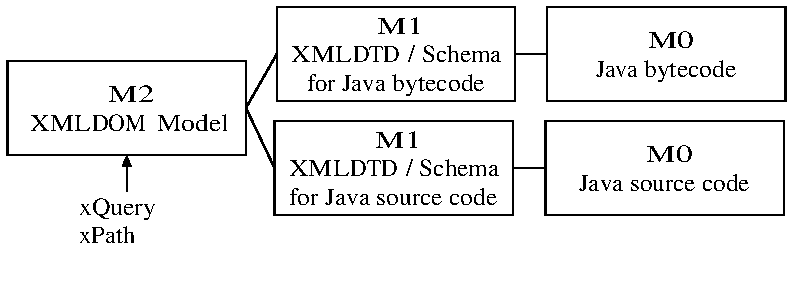
\includegraphics[width=8cm,height=!]{ch03/xml}
	\end{center}
	\caption{The XML MDA Levels}
	\label{fig:xml-mda}
\end{figure}

Working at the meta-model level unifies many specific issues that are usually important to be ignored. For the example of \fig{fig:xml-mda}, the XML queries will be more useful if they refer to the information from the M1 level models. Elements of the M1 models, e.g., language specific features, can be explored in a joinpoint model to allow more semantically rich pointcuts. This is not possible when working with the M2 level elements. However, queries specialized for one M1-level model cannot be used for another M1-level model.

%\item \textit{Arbitrary extension points.} Generic AOP engines help with declarative specification of joinpoints and with implicit meta-programming changes. The advice code itself \see{ch2:aop} can be structured with any usual OO mechanism. The freedom of implementation is good for a generic transformation framework. However, \sr{sec:ooframeworks} stressed the need for well-defined extension points in product-lines, which is difficult to enforce over the aspect implementations in generic AOP engines\footnote{In theory, adding another meta-level to the AOP programming model that is, having aspects over the aspects, can help to enforce well-defined extension points. The programming model of this meta-meta-system will be difficult to be understood by humans.}.

\end{itemize}

\noindent \textbf{AOP as a replacement for DSA.} While any generic transformation system can be used to implement DSA, no generic transformation system can replace DSA. DSA promote an explicit programming style and enrich the meta-model of a language. The programmers select explicitly the context where DSA constructs will be used. AspectJ and AOP replace the explicit programming style with selection of points of interest, enabling in theory more automation. DSA preserve the domain architecture in the code. Whereas AOP, when used as a replacement for DSA, hides the domain architecture, which makes it not suitable for emulating the DSA semantics. While AOP techniques cannot replace DSA, neither can DSA replace AOP techniques. They complement each-other and could be used together in a system. AOP engines can be used to apply AOP-style modularization in a system, working over the DSA constructs.

The consequences of AOP-style modularization are outside the scope of this work. Technically speaking, matching AOP pointcuts is a mechanical process \see{sec:aop-intro}. While pointcuts are declarative, the points of interest need to be specified often as complex composed pointcuts. The shadows of complex composed pointcuts cannot be directly imagined by humans for large systems. This means, that there could be points that are matched when they should not, and vice-versa. Investment in IDE support for AspectJ can help with this regard for a particular AOP system. Other systems \cite{alpha.05} explore less fragile pointcut models to deal with evolution of source code artifacts. While this is an area of active research, the mechanical pointcut matching is still far from replacing the human search and could result in unpredictable transformation side-effects. Attributes can be used as a workaround to express complex pointcuts, that are too complicated to be expressed otherwise. AOP techniques will not be explored any more in this book. The focus will be on the DSA support with attributes, and it will be left up to the user to decide the most appropriate programming model, on a case by case basis.

\section{Proper Usage of Explicit Attributes}
\label{sec.attribute.usage}

Attributes are easy to introduce and can carry any semantics. This can lead to \textit{abuse} of AEP, when attributes are utilized to represent semantics that can be represented better with other language means. This section discusses the proper usage of explicit attributes, giving several examples of inappropriate practices.

\subsection{When to Annotate?}

Every program element can be decorated with explicit attributes. There are natural ways to define the semantics of abstract software models in all programming languages. The OO language abstractions are usually easier to use than the explicit attributes, and are also better statically checked by the language compiler with no additional effort on the part of the developer. The following principle summarizes the first guideline for properly using explicit attributes.  

\begin{principle}
\label{pri:tagUsage}
Explicit attributes should be used to decorate an entity, when there is no simpler natural representation of the intended semantics, supported by the hosting language.
\end{principle}

\noindent The term \textit{natural} is intuitive \cite{mozart.04}, and so is the usage of tags to denote extended semantics. Everything, that can be done with attributes, can also be done without them in a Turing complete \cite{automata.2001} language. According to the principle~\ref{pri:tagUsage}, attributes help to reduce the accidental complexity, and to make the abstractions easier to introduce and implement. Several alternatives how to use explicit annotations are possible and have already been used, however, not all of them follow the principle~\ref{pri:tagUsage}, as illustrated by the examples below:

\begin{itemize}
\item Attributes can be used to decorate any element if it is allowed by the language grammar. In an OO language, decorating a 'Car' object with a 'color' tag can be more naturally implemented with a field attribute of the class 'Car'. In .NET C\# \cite{www.dotnet} decorating a structure with a custom attribute 'class' to denote OO class semantics makes no sense, given that the available 'class' keyword is the natural choice.

\item Explicit attributes can be used to augment programming languages with new constructs in a convenient way. Decorating a structure with a custom attribute 'class' makes sense in the ANSI C language to denote a class. Attributes enable customization  of a language without changing its grammar. For example, using marking interfaces to translate marked UML class diagrams to source code results in a large number of interface derivations to represent multiple tag values, as was shown in \sr{attributes}. It is more natural to deploy an attribute-based approach.

\item Non-consistent designs also exist. For example, a serializable object can be distinguished at the run-time\footnote{For example, to be able to serialize an object instance to be sent over the network during remoting \cite{dnet.remoting}.} if its class implements a required serializable marking interface. It adds nothing semantically to use both an explicit attribute and a marking interface \cite{design.attrib} to decorate a class.
%
However, implementing the serialization in .NET requires both an interface and an attribute, favoring the attribute for generation, and using the interface for the required serialization methods that need to be implemented\footnote{In practice, this design makes sometimes sense, because it reuses as much of the existing language abstractions as possible, rather than relying only on generation techniques based on attributes.}.

\item Explicit attributes can be used to represent the declared model of an application, by defining \textit{explicit hooks} \cite{java.compost} where code can be inserted. What \textit{declared model} means is a relative concept. A class definition, marked with an additional 'enterprise' attribute, contains more semantics than a class definition without this attribute. However, as shown in \fig{fig:convert}, the implicit program model can be made automatically explicit with attributes, without adding any semantics to the design.

\begin{figure}[ht]
\begin{center}
\begin{minipage}[t]{8cm}
		\begin{scriptsize}
		\begin{lstlisting}[numbers=left,language=Java,frame=leftline]{}
class WebService1 { public void Method1() {...} }
 
// goes to:

[Class(Name="WebService1")]
class WebService1 {
    [Method(Name="Method1", Modifiers="Public", ReturnType="void")]
    public void Method1() {...}
}
\end{lstlisting}
		\end{scriptsize}
		\end{minipage}
	\end{center}
	\caption{Converting the Implicit Model to an Explicit Model}
	\label{fig:convert}
\end{figure}

This means that the mere existence of explicit attributes does not show the existence of a meaningful declared model, upon which one can reason about the application's components.

\item Attribute decorations are local. It makes few sense to use local attributes for introducing global system-wide functionality. For example, local attribute decorations are used in \cite{bodden.04} to check global properties at run-time. Placing the same code in a separate module, would be more suitable and would cut in half the implementation effort. If the checked conditions are local in scope, existing Java 1.5 assertion statements would make more sense.

\end{itemize}

\subsection{What can be Annotated?}
\label{when.annotate}

It may seem that in an attribute enabled language everything can be decorated. However, the \textit{identifiable elements} of a program are different, in different representations. Sometimes the structural elements of a program, e.g., namespaces and classes, are invisible when source code is compiled to a binary file. It should be properly clarified what could be decorated, and how long this decoration is about to last. The following principle summarizes the right targets that be annotated:

\begin{principle}
\label{pri:tagTarget}
Only entities that exist and can be manipulated in a given context, can be decorated with attributes.
\end{principle}

\noindent The generic term \textit{'entity'} was used on purpose. An 'entity' is whatever can be distinguished in some way from the rest of the environment. It can be a class, a method, an object, a thread, a 'for' loop etc. 
The 'entities' have to exist in the context where the annotation is applied, and when it is interpreted. A 'for' loop exists in the AST of the source code and can be decorated. But the 'for' loop does not exist in the same form in the binary output of a compiler. Therefore the 'for' loop attributes cannot be preserved in that binary representation. Another example, is the possibility to annotate object instantiation in the source code level, because the line and the syntax are known. At run-time, an object can be decorated immediately after it is created, but the instantiation process itself cannot be decorated. 

As a consequence of this principle, there are three different contexts, where explicit annotations can be applied:

\begin{itemize}
\item \textit{Source-code level} - Attributes can decorate structural elements (e.g., classes and methods) and behavioral elements (e.g., loops and conditionals). Attributes can be processed by a preprocessor tool, or by the front-end phase of a compiler. Attributes can also be preserved for later use in the binary meta-data. However, many source-code level attributes that support code generation (e.g., used to introduce new class fields) should be processed partially or completely before or during compilation \seec{ch04}. Other source-code level attributes that decorate elements, that will not exist any more as separated entities in a binary (e.g., \textit{for} loops), need to be fully processed before compilation.

The attribute specifications in both .NET\cite{www.dotnet} and Java \cite{www.java.meta} state that attributes do not change the semantics of the code they decorate. This means that a component decorated with attributes should be able to be compiled and used even though the attributes are not processed. In practice there are many exceptions to this rule. Components decorated with attributes usually cannot be used, unless the attributes are properly processed, given that the attributes change the semantics of the component, or the semantics of the context \cite{.net.context.attrib} it lives in\footnote{That is, the attributes are an integral part of the overall semantics of a component.}. In other cases, attributes can be used to introduce fields or methods that are used by the rest of the code. Such scenarios arise often when attributes are used to drive code generation. In these cases, the component cannot compile without processing first the attributes.

\item \textit{Binary level} - Not all languages offer this possibility. In real binaries, the structural source code information is not present. The source-level equivalent entities are either not preserved, or are blurred in undeterminable ways by various semantically-equivalent compiler optimizations \cite{muchnick.97}. Meta-data enriched pseudo-binaries found in languages, such as Java and .NET, save the structural information of the source code AST inside the binary \see{sec.gaast}. In such languages, the annotation of the structural elements is preserved during compilation and can be accessed after the compilation, or at the run-time, by using reflective introspection. For example, Soot \cite{soot.00} can statically explore and modify the Java bytecode format.

\item \textit{Run-time level} - New entities exist at run-time that are not found in the source code or binaries. For example, in the source code level there are class definitions and object instantiations instructions. The real objects exists only at run-time. The same holds true for threads and virtual methods.
%
The need for attributes at run-time can be easy emulated with additional object attributes\footnote{The \textit{'Variable State'} pattern \cite{gamma.eclipse.04} can be used for specific objects or a lookup (hash) table for all objects indexed by the object.}, and will not be explored any more in this book\footnote{Using reflection at run-time to manipulate attributes is a case of binary-level attributes, and not of the run-time level attributes.}.
\end{itemize}

These contexts differ in the amount of static or dynamic information that is available. Different language technologies also differ in the amount of the information that is made available in each context. Java annotations \cite{www.java.meta} make these contexts explicit. A Java annotation can have source, binary, or virtual machine lifetime. For example, the \texttt{@Re\-ten\-tion(\-Re\-ten\-tion\-Po\-li\-cy.\-RUN\-TI\-ME)} meta-attribute denotes that a given attribute should be preserved during the execution by the Java virtual machine.




\cendsection{Chapter Summary}
\label{ch03sum}

Attributes are a lightweight language extension used to introduce custom domain-specific abstractions (DSA). Attribute-based DSA support a declarative programming model for product-line development. Attribute families organize the attributes in nested name spaces corresponding to the domain assets. Attributes can be used to drive DSA transformation\footnote{Source to source, source to binary, binary to binary and / or binary to source.} in the language technologies that support them. An attribute enabled language provides the possibility to decorate and access the decorated AST in various (equivalent) representations of the source code.

Attribute enabled languages support more directly model-driven development (MDD) compared to other language technologies used to map UML class diagrams, such as, marking interfaces, or pseudo-syntactic marking. Attribute programming helps to preserve architectural decisions in the source code. Unlike interface based mapping and pseudo-syntactic mapping, attribute mapping closely resembles the original MDA models and provides for better extensibility and a less complex programming model for the targeted OO languages. The mapping process is also simpler. Attribute enabled languages help to close the gap between thinking in terms of models, and source code.

Attributes enable new ways to design the code. UML tags and stereotypes can model only a subset of attribute design possibilities. While mapping UML tags and stereotypes to attributes is straightforward, the reverse process is not directly supported in every case by UML. Several UML notations were investigated, that can be used to model different attribute-based scenarios. 

GAAST enabled languages make it easier to extend a general-purpose OO language with domain-specific constructs. GAAST languages offer a single uniform mechanism to introduce custom extension. GAAST languages  serve as a convenient alternative to extensible compilers, for implementing attribute-based DSA. GAAST languages do not require changing and maintaining the front-end tools of the compiler. If the GAAST technology is supported by the language vendor, it becomes easy to introduce AEP in an existing project, and to maintain attribute-transformers in the long term. Languages, such as .NET and Java 1.5, already offer a lot of support for GAAST-like transformations.

Attributes should be used carefully to enhance or replace software abstractions that are already available in a language. Adding attributes is easily, however, just using attributes \textit{per se} adds no semantic value to the source code model. The set of the used attributes and their scope validity should be carefully selected, based on the domain concerns. Attributes can be preserved in various representations of the source code or the binary, if the language technology allows it. Depending on the interpretation scope, attributes can be used at (pre) compile time, after compilation, or at run-time.
